%Chapter 5
\chapter{An Adaptive Multimodal GUI Framework using LLMs}
\label{ch:chapter5}

\section{Introduction to an Adaptive Smart Home Controller}
The Adaptive Smart Home Controller \footnote{The codebase containing implementation and evaluation data of this thesis can be found at: \url{https://github.com/YarneD-1952226/A-Multimodal-AI-Driven-GUI-Framework-for-Dynamic-User-Adaptation}} is the practical proof-of-concept used to implement and validate the multimodal AI-driven GUI framework presented in this thesis. It serves as a concrete example of how the framework’s concepts, introduced in Chapter~\ref{ch:chapter3}, can be applied in a real, interactive application. The Smart Home Controller simulates the control of typical household devices such as lights, thermostats, and door locks. While the devices themselves are virtual, the process of capturing inputs, interpreting them through the backend with user profiles and history, and applying adaptive changes to the interface is authentic and functionally representative of a real deployment.

The choice for a smart home context was deliberate. It offers a relatable and real-life use case structured set of interaction scenarios that cover a range of UI components, buttons, sliders, text elements which are central to accessibility-focused adaptations. Furthermore, it reflects real-world situations where users may have diverse abilities and input preferences. For example, a motor-impaired user might need larger buttons to avoid frequent miss-taps, while a visually impaired user may benefit from higher-contrast modes and enlarged text. By embedding these scenarios into a single, unified application, the Smart Home Controller provides a manageable but representative testbed for the framework’s adaptive capabilities.

The system adheres to the three-layer architecture established in earlier chapters. The frontend layer, implemented in Flutter (\texttt{adaptive\_ui\_app.dart}), renders the interface, captures user interactions, and applies adaptation instructions as they are received from the backend. The Input Adapter Layer (\texttt{adaptive\\\_ui\_adapter.dart}) acts as a middleware component, converting raw inputs from multiple modalities into the framework’s JSON-based event format and ensuring user profiles are retrieved or updated before events are transmitted. The backend layer (\texttt{backend.py}), built with FastAPI, Gemini API and MongoDB, implements the Smart Intent Fusion (SIF) process. This includes both deterministic, rule-based adaptations and multi-agent LLM-driven reasoning (MA-SIF), combining event data, user profiles, and interaction histories to produce targeted adaptation actions.

It is important to note that this first iteration does not yet incorporate every capability described in the framework’s long-term vision. Certain modalities, such as gesture recognition, are currently simulated through mock events to keep the implementation focused on the adaptation pipeline rather than input hardware integration. Throughout this chapter, each component is discussed in detail, with a clear distinction made between fully implemented functionality, simulated elements, and features that remain as future work.

\section{Development Environment}
The development environment for the Adaptive Smart Home Controller was chosen to support rapid prototyping, cross-platform deployment, and straightforward integration with the multimodal adaptation framework described in earlier chapters. It needed to provide a fast feedback loop during implementation, flexibility in UI design, and robust backend capabilities to support real-time Smart Intent Fusion. The final setup reflects a balance between practical constraints such as available hardware, time and technical requirements namely WebSocket support, database persistence, and LLM integration.

Flutter was selected for the frontend because of its ability to produce visually consistent applications across desktop, mobile, and web from a single codebase. The framework’s reactive UI model and composable widget system made it straightforward to create adaptive components whose properties such as size, color, and layout can be updated dynamically in response to backend instructions. Flutter’s hot reload feature also significantly reduced iteration time, which proved essential for testing the frequent, small adjustments needed when refining adaptation behaviors.

The backend is implemented in Python using FastAPI, chosen for its simplicity, asynchronous request handling, and native WebSocket support. FastAPI’s lightweight structure allowed the project to keep the adaptation pipeline transparent and easily modifiable, while still offering the performance needed for real-time interactions. MongoDB was selected as the database because its document-based structure aligns directly with the JSON contracts used throughout the framework. It stores user profiles, interaction histories, and adaptation logs without the need for complex schema migrations, making it well-suited for iterative development.

Development and primary testing took place on macOS 15.6, with additional runs on Windows 11 to confirm cross-platform compatibility. Both environments used Visual Studio Code with the Flutter and Dart plugins for frontend work, and Python tooling for backend development. This combination made it possible to run and debug both layers side-by-side, with the frontend communicating directly to a locally hosted backend via WebSocket and HTTP.

For clarity, the main environment components were as follows:
\begin{itemize}
    \item \textbf{Operating System:} macOS 15.6 (primary), Windows 11 (secondary testing)
    \item \textbf{Frontend Framework:} Flutter SDK 3.7.0 or higher
    \item \textbf{Programming Languages:} Dart 2.19.0+ (frontend), Python 3.9+ (backend)
    \item \textbf{Backend Framework:} FastAPI with Uvicorn ASGI server
    \item \textbf{Database:} MongoDB 6.0+ for persistent profile and interaction history storage
    \item \textbf{IDE:} Visual Studio Code with relevant Flutter/Dart and Python extensions
    \item \textbf{Communication:} WebSocket for real-time adaptation updates, HTTP for profile management and batch operations
    \item \textbf{Version control:} Git, with the repository hosted on GitHub for collaboration and version tracking.
\end{itemize}

While this configuration is sufficient for the current implementation, it is also designed to be portable. The backend can be deployed to cloud environments without modification, and the frontend can target iOS, Android, or desktop platforms simply by recompiling or adjusting the build configuration. This flexibility ensures that the same codebase can serve as both a research prototype and a potential foundation for future production-ready systems.

% implementation details
\section{Frontend (Flutter): Adaptive Smart Home Controller}
The frontend of the Adaptive Smart Home Controller is implemented in Flutter and serves as the primary user-facing component of the framework. Its role is to render the interface, capture user interactions across multiple modalities, and apply adaptation actions received from the backend in real time. Although the backend is responsible for reasoning about what adaptations to make, the frontend is where these adaptations become visible to the user and directly influence usability.

\subsection{Responsibilities \& Data Flow}
The Flutter frontend (\texttt{AdaptiveSmartHomeApp} $\rightarrow$ \texttt{SmartHomeScreen}) renders the device cards, captures user interactions (live touch; voice/gesture mocked), and applies backend-issued adaptations in real time via a WebSocket callback. The \texttt{AdaptiveUIAdapter} is constructed with a user ID and a callback; when the backend responds with a list of \texttt{UIAdaptation} items, the frontend updates reactive state maps and triggers lightweight animations. (Figure~\ref{fig:frontend_data_flow})

\begin{figure}[h]
\centering
\begin{tikzpicture}[node distance=1.6cm,>=latex,rounded corners,thick]
\tikzstyle{box}=[draw, rounded corners, align=center, minimum width=3.4cm, minimum height=1.0cm]
\node[box] (ui) {Flutter UI\\(text, sliders, buttons)};
\node[box, right=2.6cm of ui] (adapter) {Input Adapter\\(\texttt{Event} JSON)};
\node[box, right=2.6cm of adapter] (backend) {Backend\\(SIF/MA-SIF)};
\node[box, below=1.4cm of adapter] (adapt) {\texttt{UIAdaptation[]}};
\draw[->] (ui) -- node[above]{user event} (adapter);
\draw[->] (adapter) -- node[above]{WebSocket} (backend);
\draw[->] (backend) -- node[right, xshift=6mm]{WS reply} (adapt);
\draw[->] (adapt) -- node[left,xshift=-4mm]{\texttt{applyAdaptations()}} (ui);
\end{tikzpicture}
\caption{Frontend data flow: events to adapter; adaptations back to UI.}
\label{fig:frontend_data_flow}
\end{figure}

\subsection{UI Composition \& State Model}
The UI is a scrollable list of device cards with minimalist controls each representing a smart home device such as a lamp, thermostat or a door. These cards contain core interactive elements, including buttons for on/off actions, sliders for settings such as temperature, and labels for contextual information. (Figure \ref{fig:ui_overview})

\begin{figure}[H]
\centering
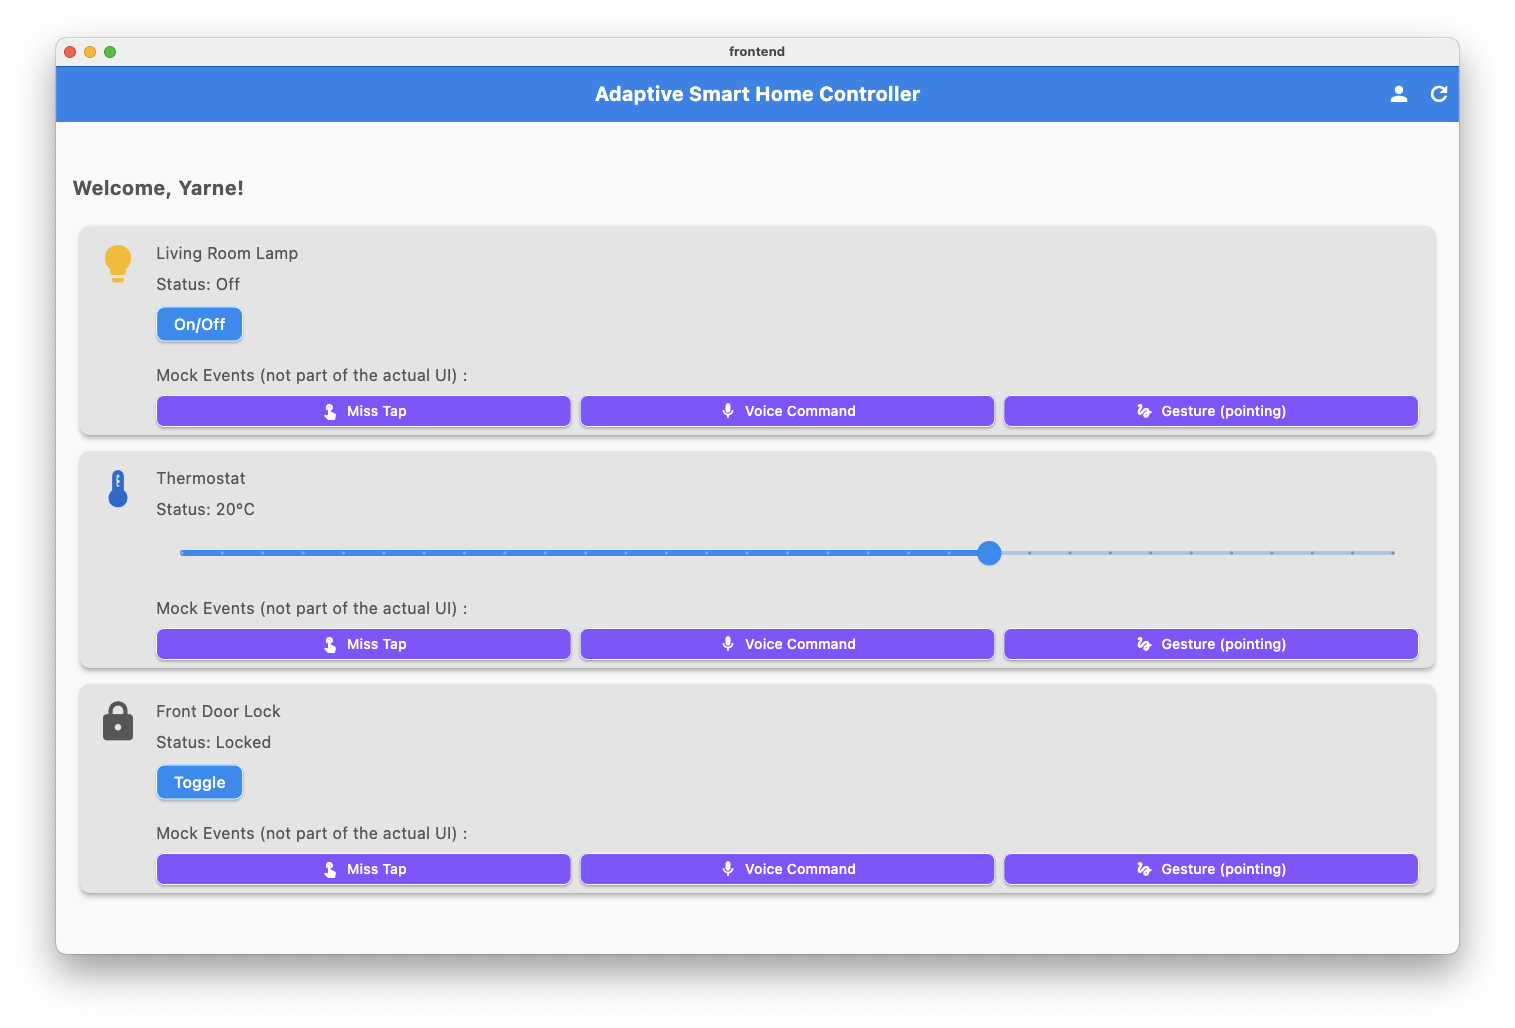
\includegraphics[width=.9\linewidth]{images/fig_ui_overview.png}
\caption{Smart Home Controller UI: scrollable device cards (Lamp, Thermostat, Lock) with minimalist controls and the mock event row (\emph{Miss Tap}, \emph{Voice Command}, \emph{Gesture}).}
\label{fig:ui_overview}
\end{figure}

The UI is intentionally minimalist, focusing on clarity and accessibility. Each device card (Lamp, Thermostat, Lock) presents its controls in a clean, uncluttered layout: large buttons for toggling states, sliders for adjustments, and concise status labels. The design prioritizes high visual contrast and generous spacing, making it easier for users with motor or visual impairments to interact. Adaptations such as increased button size, font scaling, or contrast changes are immediately reflected in the UI, with smooth animations to reinforce feedback. A persistent mock event row below each card allows users (or testers) to simulate miss-taps, voice commands, or gestures, demonstrating how the interface responds and adapts in real time. This modular structure ensures that accessibility enhancements are both visible and intuitive, supporting a wide range of user needs without overwhelming the interface.

\subsection{Event \& Adaptation Contract}
\label{sec:event_adaptation_contract}
\paragraph{Event (frontend$\rightarrow$backend).} Events carry modality and UI context:
\begin{lstlisting}[language=json, basicstyle=\ttfamily\small, caption={Event structure}]
{
  "eventType": "miss_tap", // e.g., touch, voice, gesture, miss_tap, ...
  "source": "touch", // modality
  "target": "lamp", // lamp | thermostat | lock
  "metadata": { "UI_element": "button" } // or slider, + command/gesture fields
}
\end{lstlisting}
\noindent\emph{Note.} The Dart \texttt{Event} uses camelCase fields (e.g., \texttt{eventType}, \texttt{targetElement}); the adapter serializes to snake\_case for the JSON contract.

This event will later be enriched with other required fields in the Input Adapter Layer, such as \texttt{timestamp} and \texttt{user\_id}.

\paragraph{Adaptation (backend$\rightarrow$frontend).} The backend replies with a list of atomic actions:
\begin{lstlisting}[language=json, basicstyle=\ttfamily\small, caption={Adaptation example actions}]
[
  { "action": "increase_button_size", "target": "lamp", "value": 1.2 },
  { "action": "increase_font_size", "target": "all",  "value": 1.15 },
  { "action": "increase_contrast", "target": "all" },
  { "action": "show_tooltip", "target": "lamp", "value": "Try a longer press" }
]
\end{lstlisting}

Adaptations received from the backend after being processed by the Input Adapter Layer are applied immediately using Flutter’s reactive state management, This is handled in the \verb|applyAdaptations(...)| callback function. For example, a \texttt{increase\_button\_size} action triggers an \texttt{AnimatedScale} widget update, enlarging the targeted button over a short animation to make the change more noticeable without disrupting the user’s flow. Similarly, a \texttt{increase\_contrast} action adjusts the application’s color scheme by updating theme parameters, while text-related adaptations update font sizes dynamically. Furthermore, when these adaptations reach the frontend, a brief highlight at the top of the application, indicates the changes being applied. This direct mapping between adaptation actions and Flutter widget properties allows the frontend to respond flexibly to a wide range of changes without requiring hardcoded layouts. See Table~\ref{tab:frontend-adapt-mapping} for details.

\begin{table}[H]
\centering
\caption{Adaptation-to-widget mapping (from \texttt{applyAdaptations}).}
\begin{tabular}{llp{7.8cm}}
\toprule
\textbf{Action} & \textbf{Target} & \textbf{Effect in UI} \\
\midrule
\texttt{increase\_button\_size} & device or \texttt{all} & Scales button via \texttt{buttonScales[target]} (animated). \\
\texttt{increase\_button\_border} & device or \texttt{all} & Doubles border thickness in \texttt{elementBorders}. \\
\texttt{increase\_slider\_size} & device or \texttt{all} & Multiplies slider scale in \texttt{sliderSizes}. \\
\texttt{increase\_font\_size} & (global) & Multiplies all entries in \texttt{fontSizes}. \\
\texttt{increase\_contrast} & (global) & Switches to high-contrast theme via \texttt{\_switchToHighContrastTheme()}. \\
\texttt{adjust\_spacing} & device or \texttt{all} & Scales spacing in \texttt{elementSpacing}. \\
\texttt{show\_tooltip} & device & Floating \texttt{SnackBar} with helper text. \\
\texttt{switch\_mode} & (global) & Records navigation-mode change (placeholder for future). \\
\texttt{trigger\_button} & lamp/lock & Toggles \texttt{deviceStatuses} (\emph{On/Off}, \emph{Locked/Unlocked}). \\
\texttt{simplify\_layout} & (global) & Sets \texttt{simplifiedLayout=true} to reduce clutter. \\
\bottomrule
\end{tabular}
\label{tab:frontend-adapt-mapping}
\end{table}

\subsection{Responsiveness \& Feedback}
While awaiting adaptations, the active card displays a rotating gradient border implemented via the \texttt{\_AnimatedGlowBorder} widget. This subtle animation serves as a visual indicator of system latency, signaling to users that their input is being processed and an adaptation is forthcoming. By using a non-intrusive glowing effect, the interface maintains user engagement without causing distraction or interrupting ongoing interactions (see Figure~\ref{fig:glow}). This approach is particularly beneficial for accessibility, as it provides clear feedback for users who may rely on visual cues to understand system status.
\begin{figure}[H]
\centering
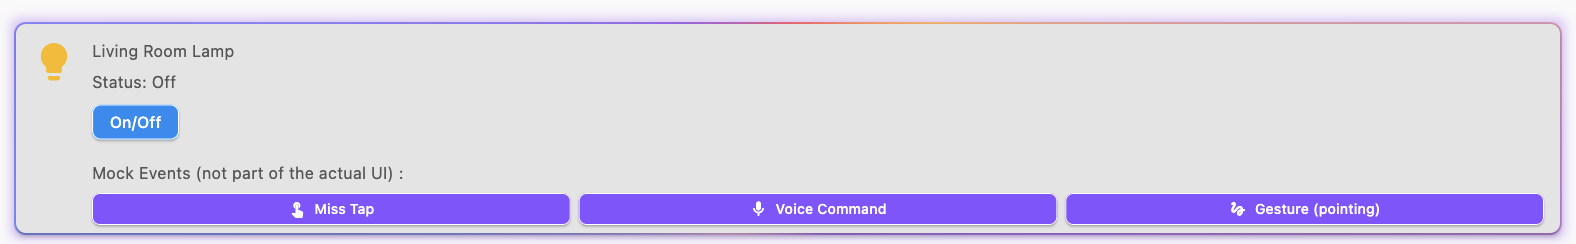
\includegraphics[width=1\linewidth]{images/fig_glow_border.png}
\caption{Loading indicator: rotating gradient card border while waiting for backend.}
\label{fig:glow}
\end{figure}

\subsection{Profile Bootstrap \& Editing}
On first run, the frontend checks if a profile exists; if not, it creates a default profile and persists it via the adapter. A bottom-sheet editor (\texttt{ProfileEditorSheet}) allows the ability to edit accessibility flags and UI preferences (font size, button size) of the user, see figure~\ref{fig:fig_profile_editor}, then calls \texttt{updateProfile(...)}.

\begin{lstlisting}[basicstyle=\ttfamily\small, caption={Profile initialization logic}]
if widget is initialized then
    adapter := AdaptiveUIAdapter(user_id, adaptation_callback)
    if adapter.checkProfile(user_id) then
        profile_data := adapter.getProfile(user_id)
        user_profile := parseProfile(profile_data)
    else
        user_profile := UserProfile(
            accessibility_needs=default,
            input_preferences=default,
            ui_preferences=default,
            interaction_history=[]
        )
        adapter.updateProfile(user_profile)
end if
\end{lstlisting}

\begin{figure}[H]
\centering
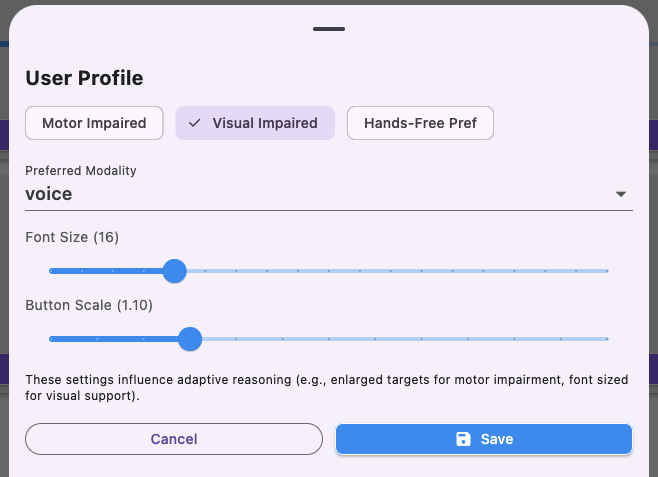
\includegraphics[width=.6\linewidth]{images/fig_profile_editor.png}
\caption{Profile editor for accessibility needs and UI preferences.}
\label{fig:fig_profile_editor}
\end{figure}

\subsection{Testing Harness: Mock Events \& Input Capture}
To validate the end-to-end pipeline without physical input hardware, a mock panel triggers \emph{miss tap}, \emph{voice command}, and \emph{gesture} events per device. Each button constructs an \texttt{Event} with modality, target, and UI context and sends it via \texttt{adapter.sendEvent(...)}. This keeps the architecture ready for real speech/gesture modules later, while staying reproducible for the study.

When a user presses on an mockup event in the test panel underneath each device, the frontend captures the event along with metadata such as the element’s type for UI context, the interaction type, and any other relevant parameters. This data is sent through the Input Adapter Layer, which standardises the event into the framework’s JSON contract before forwarding it to the backend via WebSocket. The choice of WebSocket ensures that adaptations can be returned and applied in near real time, a critical requirement for maintaining a smooth user experience in accessibility scenarios. The power of the framework lies in the ability to set the \texttt{event\_type}, \texttt{source}, and others, dynamically based on user interactions, since the backend will use LLM-reasoning to interpret these events in context. While the fields are bound by the JSON contract to standardise events (for modularity and consistency), the actual values can be highly contextual and dynamic.

\textbf{Input Capture}: The frontend layer captures raw inputs from multiple modalities, including touch, voice, and gestures. Each modality is handled through specific Flutter widgets and event listeners:
\begin{itemize}
    \item \textbf{Touch}: Taps or miss-taps on buttons/sliders, detected via Flutter’s \verb|GestureDetector| or \verb|onPressed| callbacks. Miss-taps are mocked but extensible to hover or real misstap detection like \verb|MouseRegion| or \verb|Listener| widgets, to create a "detection bounding box".
    \item \textbf{Voice}: Commands like “Turn on lamp” or “Unlock door”, mocked for this thesis but extensible to libraries like \verb|speech_to_text| or Web Speech API.
    \item \textbf{Gestures}: Hand movements (e.g., point, swipe) via mock events, with future support for MediaPipe.
\end{itemize}

\subsection{Summary}
Overall, the Adaptive Smart Home Controller (\texttt{adaptive\_ui\_app.dart}) demonstrates how the frontend layer of the framework can be implemented in a way that is both platform-independent and responsive to dynamic adaptation instructions. By separating UI rendering from adaptation logic and using the Input Adapter Layer as a bridge, the application remains modular, making it easier to extend or replace individual components without affecting the overall system.

% implementation details and extensibility eye tracking
\section{Input Adapter (Dart): Transport, Serialization \& Adaptation Callback}
The adapter bridges the Flutter frontend and the SIF backend by (i) serializing internal \texttt{Event} objects into the JSON event contract, (ii) handling low-latency transport via WebSocket for adaptations, and (iii) managing user profiles over HTTP. This section focuses on the concrete implementation in \texttt{adaptive\_ui\_adapter.dart}: the class surface, serialization choices, transport lifecycle, and the \texttt{onAdaptations} callback function into the frontend. See Chapter~\ref{ch:chapter3} for the high-level event schema and field definitions.

\subsection{Class Overview}
\begin{figure}[H]
\centering
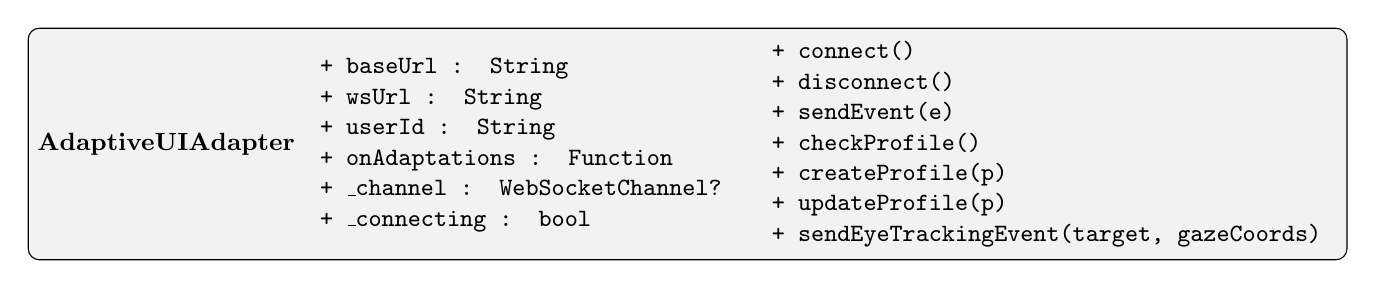
\begin{tikzpicture}[
    font=\small,
    class/.style={draw, rounded corners, fill=gray!10, minimum width=4.5cm, minimum height=2.2cm},
    attr/.style={font=\ttfamily\scriptsize},
    meth/.style={font=\ttfamily\scriptsize, text width=4.2cm, align=left}
]
\node[class] (adapter) {
    \textbf{AdaptiveUIAdapter}
    \vspace{2pt}
    \begin{tabular}{l}
        \texttt{+ baseUrl : String} \\
        \texttt{+ wsUrl : String} \\
        \texttt{+ userId : String} \\
        \texttt{+ onAdaptations : Function} \\
        \texttt{+ \_channel : WebSocketChannel?} \\
        \texttt{+ \_connecting : bool} \\
    \end{tabular}
    \vspace{2pt}
    
    \vspace{2pt}
    \begin{tabular}{l}
        \texttt{+ connect()} \\
        \texttt{+ disconnect()} \\
        \texttt{+ sendEvent(e)} \\
        \texttt{+ checkProfile()} \\
        \texttt{+ createProfile(p)} \\
        \texttt{+ updateProfile(p)} \\
        \texttt{+ sendEyeTrackingEvent(target, gazeCoords)} \\
    \end{tabular}
};

\end{tikzpicture}
\caption{Simplified UML-like diagram for \texttt{AdaptiveUIAdapter}.}
\label{fig:adaptive-ui-adapter}
\end{figure}

In the current implementation (Figure~\ref{fig:adaptive-ui-adapter}), the adapter intercepts mock events generated by the frontend, such as missed button presses, missed slider adjustments, or simulated voice commands. Each event is enriched with metadata, including the user’s identifier, a timestamp, the type of interaction, and any target element references. The adapter then converts this information into the JSON event contract, further defined in Chapter~\ref{ch:chapter3}, which serves as the standard interface between the frontend and backend. This contract includes fields for event type, source modality, target element, coordinates if applicable, confidence level, time stamp, user\_id and additional metadata such as the spoken command in the case of voice input.

\subsection{Internal Representations of Event, Adaptation and User Profiles}
The adapter defines core Dart classes for representing interaction events, user profiles, and adaptation actions. The \texttt{Event} class encapsulates all relevant fields such as event type, source modality, target element, etc., ensuring every interaction is consistently structured and easily serializable to the backend’s JSON contract (see figure \ref{fig:adapter-classes} for schema details). Similarly, \texttt{UIAdaptation} models adaptation instructions received from the backend, while \texttt{UserProfile} maintains accessibility needs, preferences, and recent history. These unified data structures guarantee reliable, type-safe communication between frontend and backend, simplify integration, and support extensibility for future modalities or adaptation types.

\begin{figure}[H]
\centering
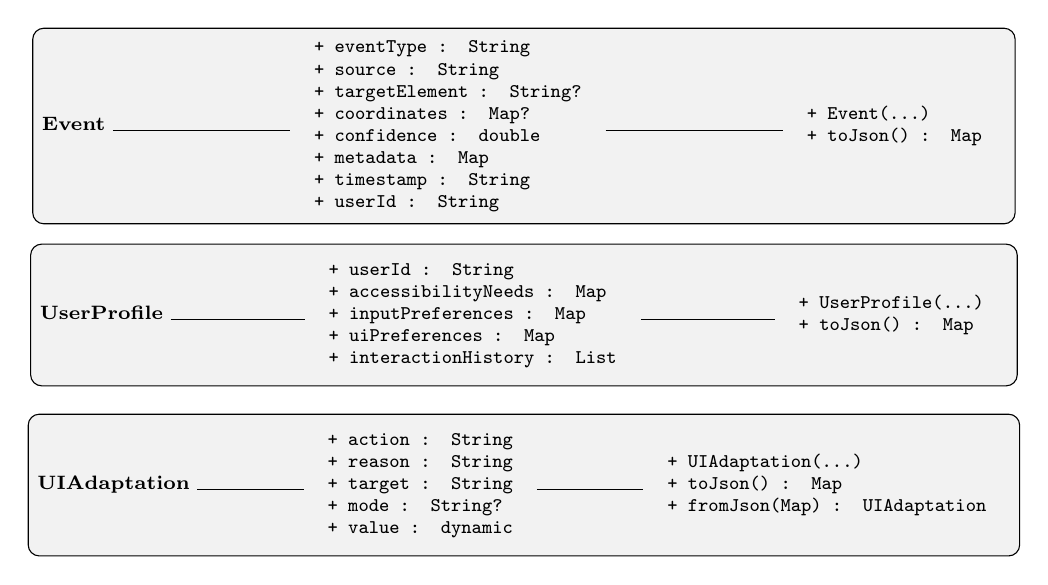
\begin{tikzpicture}[
    scale=0.6, % reduced from 0.8 for smaller diagram
    font=\scriptsize,
    class/.style={draw, rounded corners, fill=gray!10, minimum width=3cm, minimum height=1.8cm, align=left},
    attr/.style={font=\ttfamily\tiny},
    meth/.style={font=\ttfamily\tiny}
]

% Event class
\node[class] (event) at (0,0) {
    \textbf{Event}
    \rule{2.25cm}{0.3pt}
    \begin{tabular}{l}
        \texttt{+ eventType : String} \\
        \texttt{+ source : String} \\
        \texttt{+ targetElement : String?} \\
        \texttt{+ coordinates : Map?} \\
        \texttt{+ confidence : double} \\
        \texttt{+ metadata : Map} \\
        \texttt{+ timestamp : String} \\
        \texttt{+ userId : String} \\
    \end{tabular}
    \rule{2.25cm}{0.3pt}
    \begin{tabular}{l}
        \texttt{+ Event(...)} \\
        \texttt{+ toJson() : Map} \\
    \end{tabular}
};

% UserProfile class
\node[class] (profile) at (0,-4) {
    \textbf{UserProfile}
    \rule{1.7cm}{0.3pt}
    \begin{tabular}{l}
        \texttt{+ userId : String} \\
        \texttt{+ accessibilityNeeds : Map} \\
        \texttt{+ inputPreferences : Map} \\
        \texttt{+ uiPreferences : Map} \\
        \texttt{+ interactionHistory : List} \\
    \end{tabular}
    \rule{1.7cm}{0.3pt}
    \begin{tabular}{l}
        \texttt{+ UserProfile(...)} \\
        \texttt{+ toJson() : Map} \\
    \end{tabular}
};

% UIAdaptation class
\node[class] (adaptation) at (0,-7.6) {
    \textbf{UIAdaptation}
    \rule{1.35cm}{0.3pt}
    \begin{tabular}{l}
        \texttt{+ action : String} \\
        \texttt{+ reason : String} \\
        \texttt{+ target : String} \\
        \texttt{+ mode : String?} \\
        \texttt{+ value : dynamic} \\
    \end{tabular}
    \rule{1.35cm}{0.3pt}
    \begin{tabular}{l}
        \texttt{+ UIAdaptation(...)} \\
        \texttt{+ toJson() : Map} \\
        \texttt{+ fromJson(Map) : UIAdaptation} \\
    \end{tabular}
};

\end{tikzpicture}
\caption{High-level class diagram for Input Adapter Layer data structures.}
\label{fig:adapter-classes}
\end{figure}

\subsection{Transport \& Profile Management}
Before forwarding an event, the adapter queries the backend via HTTP to check whether a profile exists for the given user. If no profile is found, it prompts the frontend to initiate a profile creation request, using default parameters or pre-filled accessibility preferences where available. This mechanism prevents situations where adaptation requests are processed without the necessary user context, which could lead to ineffective or even counterproductive UI changes.

Communication with the backend is handled primarily through WebSocket for low-latency adaptation feedback. HTTP requests are used for profile management, batch operations, and other non-real-time interactions. This division ensures that profile updates and administrative tasks do not interfere with the responsiveness of live adaptations, see table \ref{tab:adapter_endpoints} for details.

\begin{table}[H]
\centering
\caption{Adapter endpoints used by \texttt{adaptive\_ui\_adapter.dart}.}
\begin{tabular}{lll}
\toprule
Purpose & Method/Proto & Path \\
\midrule
Realtime adaptations & WebSocket & \verb|/ws/adapt| \\
Check profile exists & GET & \verb|/profile/{user_id}| \\
Create profile       & POST & \verb|/profile| \\
Update profile       & POST  & \verb|/profile| \\
\bottomrule
\end{tabular}
\label{tab:adapter_endpoints}
\end{table}

\textbf{WebSocket Lifecycle \& Error Handling:}
\begin{figure}[H]
\centering
\begin{tikzpicture}[>=latex, node distance=1.8cm, on grid, auto,
  state/.style={draw, rounded corners, align=center, minimum width=2.6cm, minimum height=7mm}]
\node[state] (disc) {Disconnected};
\node[state, right=of disc,xshift=25mm] (conn) {Connecting};
\node[state, right=of conn, xshift=25mm] (open) {Open};

\draw[->] (disc) -- node{connect()} (conn);
\draw[->] (conn) -- node{onOpen} (open);

\draw[->] (open) .. controls +(0,1.0) and +(0,1.0) .. node[above]{ping/pong} (open);
\end{tikzpicture}
\caption{Adapter WebSocket lifecycle with reconnect backoff.}
\end{figure}

\noindent In \texttt{adaptive\_ui\_adapter.dart}:
\begin{itemize}
  \item On \textbf{open}: subscribe to messages and (optionally) flush any queued events.
  \item On \textbf{message}: parse JSON array/object, convert to \texttt{UIAdaptation} list, invoke \texttt{onAdaptations}.
  \item On \textbf{error/done}: close channel.
  \item \textbf{Keep-alive via ping/pong}: Keep-alive via ping/pong is handled at the protocol level; the adapter does not send explicit pings.
\end{itemize}

\textbf{Sending Events:}

When the frontend is ready to send an event, it calls the \texttt{sendEvent} function from the adapter, which enriches the event data with metadata (e.g., user\_id, timestamp), serializes it into JSON, and sends it over the WebSocket connection. 

\begin{lstlisting}[language=Dart,basicstyle=\ttfamily\small,caption={sendEvent: serialize and send over WS}]
void sendEvent(Event eventData) {
    eventData.timestamp = DateTime.now().toIso8601String();
    eventData.userId = userId;
    channel!.sink.add(jsonEncode(eventData.toJson()));
}
\end{lstlisting}

\textbf{Receiving Adaptations:}

When the adapter receives adaptations from the backend in the WebSocket channel, the adapter processes the JSON and converts them in a \texttt{UIAdaptation} list. This list is then passed to the \texttt{onAdaptations} frontend callback function. This function is responsible for updating the UI based on the received adaptation data, see Section~\ref{sec:event_adaptation_contract} for more details on this process.

\textbf{Profile Management:}

Profile management is mostly done by the frontend, with the Input Adapter Layer providing all the necessary functions and ensuring that every user interaction is contextualized with the correct accessibility preferences and history. Before sending any event to the backend, the frontend (as described earlier) checks whether a profile exists for the current user by calling \texttt{checkProfile()}. If no profile is found, it creates one using \texttt{createProfile(UserProfile p)}, which serializes the profile data and posts it to the backend. Updates to the profile, such as changes in accessibility needs or UI preferences, are handled by \texttt{updateProfile(UserProfile p)}, which issues a POST request with the updated profile JSON. These functions guarantee that the backend always receives events enriched with up-to-date user context, supporting personalised adaptation and continuous learning.

\subsection{Extensibility Example}
As proof-of-concept for the extensibility of the framework, a gaze event hook was implemented that incorporates eye-tracking data into an event. This demonstrates how easily new input modalities can be integrated into the existing architecture.
\begin{lstlisting}[language=Dart,basicstyle=\ttfamily\small,caption={Gaze event hook (testing harness)}]
void sendEyeTrackingEvent(String target, Map<String,double> gazeCoords) {
  sendEvent(Event(
    eventType: 'eye_tracking',
    source: 'gaze',
    targetElement: target,
    coordinates: gazeCoords,
    confidence: 1.0,
  ));
}
\end{lstlisting}
\textit{Note:} This can either be done in the frontend or directly in the adapter, depending on the specific requirements of the application. For demonstration purposes, the gaze event hook was implemented in the adapter, while the frontend would be a more logical place for it in a production setting.

\subsection{Summary}
The adapter is fully wired for touch events and for mocked voice/gesture events triggered from the frontend’s test panel, enabling end-to-end validation without external hardware. The adapter treats mocked and real events identically, so integrating actual speech/gesture modules later is a frontend-only change. By isolating serialization, profile checks, and transport here, the frontend stays focused on rendering, and the backend receives consistent inputs. The same adapter design can be reused in SwiftUI or other platforms with minimal changes to the method surface and JSON contract.

\section{SIF Backend Layer: Implementation of Adaptation Logic}
The backend implements the decision‑making core of the framework. It receives standardised events from the adapter, fuses them with user profiles and recent interaction history, and returns concrete adaptation actions for the frontend to apply. The service is written in Python using FastAPI, with Uvicorn for serving requests and MongoDB for persistent storage of profiles and logs. WebSocket is used for low‑latency, bidirectional communication during interaction, HTTP is used for profile management and auxiliary endpoints.

\subsection{Webserver layout and endpoints}
The application exposes a WebSocket endpoint, \texttt{/ws/adapt}, that accepts JSON events matching the contract introduced earlier. Each message is parsed into a Pydantic \texttt{Event} model, the user profile is loaded from MongoDB, and the event, profile, and short history window are passed to the Smart Intent Fusion routine. The resulting adaptation list is returned on the same socket, allowing the frontend to update the UI immediately. For non‑interactive operations the backend offers \texttt{POST /profile} for profile creation, \texttt{GET /profile/{user\_id}} for retrieval, and a small set of diagnostic endpoints such as \texttt{GET /full\_history} and \texttt{GET /modalities}. Profile writes use FastAPI \texttt{BackgroundTasks}, which keeps the interaction path responsive while updates are persisted asynchronously.

\subsubsection*{Startup \& Runtime}
For local runs, the service is started via a small shell script (\texttt{start\_backend\_processes.sh}) that prepares a venv, checks MongoDB, and runs Uvicorn with explicit WebSocket keepalive settings:
\begin{lstlisting}[basicstyle=\ttfamily\small,caption={Backend startup (excerpt)}]
uvicorn backend:app --reload --host 0.0.0.0 --port 8000 \
  --ws websockets --ws-ping-interval 60 --ws-ping-timeout 180
\end{lstlisting}
This configuration enables reliable long-lived WS sessions during interactive testing, and eases startup of all the different services.

\subsection{Data persistence and history management}
MongoDB stores user profiles in a \texttt{profiles} collection and event–adaptation pairs in a \texttt{logs} collection. Profiles are indexed by \texttt{user\_id} to allow direct lookups during interaction. Each time an event is processed the backend appends a compact JSON representation to the profile’s \texttt{interaction\_history}, capped to a small sliding window. This keeps the prompt context focused on recent behaviour while avoiding unnecessary growth in the database. For redundancy, a JSONL file mirrors the log entries during development, which simplifies offline inspection or debugging purposes when the database is reset.

\subsection{Smart Intent Fusion and MA‑SIF}
The fusion step supports two paths. A multi‑agent configuration, MA‑SIF, is the default. It loops over a set of specialised LLM agents, UI, Geometry, and Input, each prompted with the current event, the user profile, and a short history via runtime injection (for more details see Chapter~\ref{ch:chapter4}), defined in the \texttt{sif\_config.json}. These agents propose structured adaptations in their domain, for example increasing button size, adjusting spacing, switching input mode, or triggering a button when intent is clear. Their outputs are then passed to a dedicated Validator agent that consolidates, filters, and normalises the suggestions into a final list. The validator removes duplicates, corrects out‑of‑range values, and ensures that every adaptation conforms to the allowed action set and includes a target and either a value or a mode and more. See Table~\ref{fig:current-agent-configuration} for the current agent configuration.

A single‑agent SIF path is also available. It produces a complete adaptation list in one call and is useful when quick iteration is preferable over agent specialisation. Both paths share the same I/O schema, which keeps the frontend indifferent to which reasoning strategy is currently set to active.

\subsubsection*{Current Agent Configuration (MA-SIF balanced) (from \texttt{sif\_config.json})}
\begin{table}[H]
\centering
\begin{tabular}{p{2.1cm}p{4cm}p{4cm}p{4cm}}
\toprule
\textbf{Agent} & \textbf{Focus (examples)} & \textbf{Allowed actions} & \textbf{Model / params} \\
\midrule
UI suggestion & increase font sizes; enable contrast mode; stronger button borders; tooltips & \texttt{increase\_font\_size}, \texttt{increase\_contrast}, \texttt{increase\_button\_border}, \texttt{show\_tooltip} & \texttt{gemini-2.5-flash-lite}, temp{=}0.2, timeout{=}15\,s, thinking\_budget=0 \\
Geometry & spacing; button size; slider size; simplify layout & \texttt{increase\_button\_size}, \texttt{increase\_slider\_size}, \texttt{adjust\_spacing}, \texttt{simplify\_layout} & \texttt{gemini-2.5-flash-lite}, temp{=}0.2, timeout{=}15\,s, thinking\_budget=0 \\
Input & mode switching; trigger buttons & \texttt{switch\_mode}, \texttt{trigger\_button} & \texttt{gemini-2.5-flash-lite}, temp{=}0.2, timeout{=}15\,s, thinking\_budget=0 \\
Validator & consolidate + validate all suggestions & \emph{all actions above} & \texttt{gemini-2.5-flash}, temp{=}0.3, timeout{=}30\,s, thinking\_budget=-1 \\
\bottomrule
\end{tabular}
\caption{MA\textendash SIF agents, focus, allowed actions, and model settings (runtime configurable).}
\label{fig:current-agent-configuration}
\end{table}

\paragraph{Runtime defaults:}
\begin{itemize}
  \item \textbf{Default model settings:} 
    \begin{itemize}
        \item UI/Geometry/Input use \texttt{gemini-2.5-flash-lite} with a temperature of 0.2, a 15\,s timeout and thinking budget of 0 (no thinking).
        \item Validator uses \texttt{gemini-2.5-flash} with a temperature of 0.3, a 30\,s timeout and thinking budget of -1 (dynamic).
    \end{itemize}
  \item \textbf{Whitelisting:} Each agent is restricted to an \emph{allowed action set}; Validator allows the union set only.
  \item \textbf{Schema enforcement:} Responses must match the JSON schema (\texttt{response\_json\_schema}); non-conforming replies trigger fallback.
  \item \textbf{Low temperature + narrow prompts:} Specialist prompts reduce creative drift and injection surface.
  \item \textbf{Timeouts:} Per-agent time budgets ensure the loop returns within interaction thresholds.
\end{itemize}

\subsection{LLM invocation (Gemini)}
For each event, the backend invokes Gemini per specialist agent (UI, Geometry, Input) and then once for the Validator, in sequence. Each call is single-shot (no streaming) with a strict JSON response contract. Requests are composed as follows:

\paragraph{Request composition:}
\begin{itemize}
  \item \textbf{Context blocks}: \texttt{event\_json}, \texttt{profile\_json} (accessibility flags, preferences), and \texttt{history\_json} (recent 10 interactions). These are injected into the Agent's prompt at runtime, as mentioned earlier.
  \item \textbf{Agent preamble}: a short, role-specific instruction and focus items plus an explicit \emph{allowed action set} (whitelisting).
  \item \textbf{Output contract}: instructed to return only a JSON envelope \texttt{\{"adaptations":[...]\}} (no prose).
\end{itemize}

\paragraph{Generation configuration (per call).}
\begin{itemize}
  \item \textbf{Model/temperature}: UI, Geometry, Input use \texttt{gemini-2.5-flash-lite} at $T{=}0.2$; the Validator uses \texttt{gemini-2.5-flash} at $T{=}0.3$ (see \texttt{sif\_config.json}).
  \item \textbf{Response format}: \texttt{response\_mime\_type=application/json} with a \textbf{JSON Schema} that enforces types, fields, and that either \texttt{value} (numeric) \emph{or} \texttt{mode} (categorical) is present.
  \item \textbf{Budgets}: per-agent timeout $\approx$ 15\,s; Validator timeout $\approx$ 30\,s. Calls are sequential by design to keep rate-limits predictable and simplify partial results.
  \item \textbf{Determinism}: low temperatures, single candidate, narrow prompts; agents propose domain-scoped adaptations, Validator consolidates/filters to the final set.
\end{itemize}

\paragraph{Failure handling.}
If a specialist agent times out or returns invalid JSON, its suggestions are omitted; the Validator runs on whatever is available. If validation still fails schema checks or time outs, the backend emits the available adaptation or conservative rule-based adaptations as a fallback.

\subsection{Structured outputs and guardrails}
To reduce hallucinations and schema drift, the backend requests JSON‑typed responses from the LLM with an explicit schema and allowed actions, as described earlier in Chapter~\ref{ch:chapter4}. The prompt defines required fields, expected types, and a one‑of constraint that demands either a numeric \texttt{value} or a categorical \texttt{mode}. Agent prompts are intentionally narrow, which improves determinism. The validator prompt is broader, since it must adjust conflicting suggestions and justify final choices. Despite these controls, invalid outputs still occur occasionally. However, the schema can be enforced at two distinct levels: by the agents and by the validator. This dual-level approach makes it easier for the validator to ensure that the agents' adaptations are compliant. Furthermore, it has a defensive layer that falls back to simple rules if all LLM validation fails.
The output schema will produce an adaptation of the following format:\\
\lstinline[language=json,basicstyle=\ttfamily\small,caption={Example adaptation Format}]|{"adaptations":[{"action":"...","target":"...","value\mode":...,"reason":"...","intent":"..."}]}|

\subsection{Rule‑based fallback and resilience}
A lightweight rule engine acts as a safety net when LLM calls time out or the provider is unavailable. This rule engine comes into action when all the suggestion agents fail (no output). It covers essential accessibility behaviours, for example increasing button size after a miss‑tap, switching to voice for users flagged as motor‑impaired, or enabling high‑contrast mode for visually impaired profiles. These rules are intentionally conservative, they guarantee progress without surprising the user, and they keep the implementation usable in environments with unstable connectivity.

\subsubsection*{Fallback rules (summary)}
\begin{table}[H]
\centering
\caption{Rule triggers and conservative adaptations (fallback path).}
\begin{tabular}{p{5.7cm}p{9.2cm}}
\toprule
\textbf{Trigger} & \textbf{Adaptation(s)} \\
\midrule
Miss tap (\texttt{event\_type="miss\_tap"}) or slider miss & \texttt{increase\_button\_size} on target (default \texttt{1.3}); intent=``difficulty hitting target''. \\
Profile indicates motor impairment & \texttt{increase\_button\_size} on \texttt{all}; intent=``Improve accessibility''. \\
Profile indicates visual impairment & \texttt{increase\_contrast} on \texttt{all}; intent=``improve visibility''. \\
Voice command detected (\texttt{event\_type="voice"}) & \texttt{switch\_mode} to \texttt{voice} on \texttt{all}. \\
\bottomrule
\end{tabular}
\end{table}

\subsection{Heatmap Analysis}
Due to time constraints, heatmap analysis is not implemented. This is a potential area for future work, as understanding user interaction patterns and frequent touch points, could further enhance the system's adaptability. Heatmap analysis has a big potential in the repositioning of UI elements based on the heatmap data, this could improve accessibility for users with specific needs like gesture-based inputs. Since the repositioning of elements is not supported in this first iteration, the focus remains on immediate adaptation strategies, which made heatmap analysis out of scope.

\subsection{Latency, partial results, and error handling}
The WebSocket loop is designed to return something useful as quickly as possible. Agent calls run in sequence within short time budgets. If one agent fails to respond, the validator operates on the remaining suggestions rather than waiting indefinitely. The backend aims to keep per‑event processing below the threshold where users notice a lag on interaction, which is important for accessibility, particularly when enlarging targets immediately after an error. In practice, most adaptations are returned quickly by the smaller suggestion agents, while validation can become the slowest step in complex scenes. When validation exceeds its budget the backend returns the best available subset, then continues to append the event to the user’s history so future interactions benefit from the context.

\subsection{Security and CORS considerations}
During development the backend enables permissive CORS to simplify local testing across platforms. Profiles are keyed by \texttt{user\_id} rather than personal data. For production deployment, stricter origins, authentication, and encryption would be required. These measures are outside the scope of this prototype, but the separation of concerns in the current design makes them straightforward to add.

\subsection{Summary}
In its current form the backend delivers a complete adaptation pipeline: events arrive over WebSocket, profiles and short history windows are loaded from MongoDB, MA-SIF produces structured suggestions, a validator consolidates them, and the result is returned to the frontend within a single interaction loop. When LLM reasoning is unavailable, conservative rules ensure the interface remains usable. This combination of multi‑agent reasoning, strict schemas, and rule-based fallbacks gives the system both flexibility and reliability, which is essential for accessibility‑focused adaptations.

\section{User Profile and Context Implementation}
The user profile and context subsystem was implemented as a dedicated data service in the SIF backend, designed to persist accessibility needs, interaction preferences, baseline UI configurations, and a capped history of recent events. MongoDB serves as the primary storage layer, with the \texttt{profiles} collection indexed on \texttt{user\_id} as described earlier for constant-time retrieval during event processing.

When a new event is received via the WebSocket (\texttt{/ws/adapt}), the backend queries the profile store using the supplied \texttt{user\_id}. If no profile exists, the profile will be created and added to the MongoDB using \texttt{insert\_one} before continuing, otherwise the profile will be retrieved using \texttt{find\_one} or updated using \texttt{update\_one}, ensuring that all adaptation decisions are made in a contextualized environment. This retrieval step is synchronous, guaranteeing that the most recent committed profile is available to the reasoning pipeline before any LLM or rule-based evaluation occurs. Interaction history is maintained using MongoDB’s \texttt{\$push} with \texttt{\$slice} operators to append the incoming event while capping the array length at 10 entries for efficiency. This rolling history provides the SIF agents with temporal context, enabling progressive personalization; for example, recognising a pattern of repeated miss-taps and proactively switching to voice mode. Updates to the history are performed asynchronously to avoid blocking real-time adaptation.

Profile documents are structured as JSON as described in Chapter~\ref{ch:chapter4}, containing four key sections: \texttt{accessibility\_needs} (boolean capability flags), \texttt{input\_preferences} (preferred modality and fallback order), \texttt{ui\_preferences} (default font size, button scale and more), and \texttt{interaction\_history} (recent event log). This schema strikes a balance between simplicity and extensibility, allowing new fields to be added without migration overhead.

To optimise performance and safety, all profile mutations are atomic, relying on MongoDB transactions to prevent race conditions when simultaneous events and updates occur. Adaptation logs are stored separately in the \texttt{logs} collection and mirrored to a local \texttt{adaptation\_log.jsonl} file, supporting offline analysis and reproducibility of evaluation results. Furthermore, if a profile update is in-flight during an event, the backend uses the latest committed profile, mitigated by client-side checks (waiting for \texttt{POST /profile} success) and server-side transactions.

This implementation ensures that every adaptation decision, whether produced by a static rule or the multi-agent LLM pipeline, is grounded in the user’s persisted profile and immediate interaction context, enabling consistent, personalised, and stateful UI behaviour across sessions.

\section{Dynamic Adaptation Mechanisms Implementation}
The dynamic adaptation mechanism is the final stage in the adaptation pipeline, where decisions made by the backend are translated into immediate and visible changes in the user interface. In the current implementation, this process is tightly integrated with Flutter’s reactive widget system, allowing adaptation actions to be applied without forcing full UI rebuilds or navigation resets.

When the backend sends an adaptation list over the WebSocket connection, the frontend parses each action and routes it to the relevant UI element. Actions are defined in the strict JSON schema described earlier, containing the \texttt{action} type, a \texttt{target} identifier, a \texttt{value} or \texttt{mode}, and a human-readable \texttt{reason} and \texttt{intent} it inferred from the adaptation. This standardisation allows the same adaptation handler to process diverse actions without requiring modality-specific logic.

The framework applies a predefined set of accessibility-oriented actions (see Table~\ref{tab:frontend-adapt-mapping} for the concrete widget mappings used by the Flutter implementation).
These adaptation actions form the cornerstone of the framework’s accessibility-driven approach, addressing diverse user needs in the Adaptive Smart Home Controller. Each action is carefully designed to align with WCAG 2.1 guidelines, ensuring inclusivity for motor-impaired users (e.g., larger buttons/sliders, increased spacing), visually impaired users (e.g., high-contrast modes, highlighted borders), and hands-free users (e.g., tooltips, mode switching).

\subsection{Application Mechanics (State, Animation, Ordering)}
\begin{itemize}
  \item \textbf{State deltas.} Element-scoped actions update per-element maps (e.g., \texttt{buttonScales[target]}, \texttt{elementBorders[target]}), while global actions flip flags or theme variables (\texttt{increase\_contrast}, \texttt{switch\_mode}).
  \item \textbf{Animation semantics.} Size and spacing changes use lightweight implicit animations (\texttt{AnimatedScale}, \texttt{AnimatedContainer}) with short durations to make changes perceivable without disrupting interaction.
  \item \textbf{Ordering.} Adaptations are applied in the order received; the backend validator guarantees a coherent, non-overlapping set. On receipt, the active card’s glow border stops and controls are re-enabled.
\end{itemize}

The application of adaptations begins with a lookup to determine whether the \texttt{target} element exists in the current view. If it does, the corresponding widget state is updated directly. For example, an \texttt{increase\_button\_size} action adjusts the scale factor property of the button widget, and an \texttt{increase\_font\_size} action updates the text style parameter. Where appropriate, changes are animated using Flutter’s \texttt{AnimatedScale} or \texttt{AnimatedContainer} to make the transition noticeable without distracting the user. This animation step is particularly important for accessibility, as it helps the user understand that the interface has been modified intentionally. The loading indicator displayed around the card being interacted is now also triggered to stop playing.

Adaptations that affect the entire interface, such as \texttt{increase\_contrast} or \texttt{switch\_mode}, are handled at the application theme level. Contrast adjustments update the color palette by replacing the primary and background colors with higher-contrast alternatives, while mode switches alter the active input modality, for example switching from touch to voice. These global changes are propagated across all widgets automatically through Flutter’s state management, ensuring consistency without manually updating each element (see table~\ref{tab:adaptation-scope} for an overview).

\begin{table}[H]
\centering
\caption{Scope of adaptations in the Flutter implementation.}
\begin{tabular}{lp{9cm}}
\toprule
\textbf{Global (theme/state)} & \texttt{increase\_contrast}, \texttt{switch\_mode}, \texttt{simplify\_layout}, \texttt{increase\_font\_size (all)} \\
\midrule
\textbf{Element-scoped} & \texttt{increase\_button\_size}, \texttt{increase\_button\_border}, \texttt{increase\_slider\_size}, \texttt{adjust\_spacing}, \texttt{show\_tooltip}, \texttt{trigger\_button} \\
\bottomrule
\end{tabular}
\label{tab:adaptation-scope}
\end{table}

Not all adaptations are implemented with live modality inputs. For demonstration purposes, actions triggered by voice or gesture events are generated from simulated events in the frontend’s test panel in each device card, like was mentioned earlier. However, these simulated actions follow the same processing path as real events, which means that integrating actual input sources in the future will require no changes to the adaptation mechanism itself.

\subsection{Conflicts and Unknown Actions}
The validator resolves conflicts server-side; the frontend applies the resulting set atomically in a single frame. If duplicate actions target the same element, the last write wins within the frame. Unknown or ill-typed actions are logged and ignored, preserving UI stability.

\subsection{Real-Time Adaptation Example}
To illustrate the framework's adaptation capabilities, consider a scenario where a visually impaired user with voice preference attempts to interact with the Smart Home Controller. The user profile contains the following settings:

\begin{lstlisting}[language=json, caption={User profile for visually impaired user, shortened}]
{
    ...
    "accessibility_needs": { "visual_impaired": true },
    "input_preferences": { "preferred_modality": "voice" },
    "ui_preferences": { "font_size": 16, "button_scale": 1.1 }
}
\end{lstlisting}

\paragraph{Event Trigger:} The user attempts to activate the lamp by tapping its button but misses the target due to the button's insufficient size relative to their visual and motor coordination needs. This generates a \texttt{miss\_tap} event on the \texttt{lamp} target, which is captured by the frontend and sent through the Input Adapter Layer to the SIF backend.

\paragraph{SIF Reasoning Process:} The backend combines the miss-tap event with the user's profile and recent interaction history. The MA-SIF agents analyze the situation:
\begin{itemize}
        \item \textbf{UI Agent:} Recognizes visual impairment flags and suggests contrast and font improvements
        \item \textbf{Geometry Agent:} Identifies the miss-tap pattern and recommends button enlargement and border enhancement
        \item \textbf{Input Agent:} Notes voice preference and triggers the intended action while suggesting mode awareness
        \item \textbf{Validator Agent:} Consolidates suggestions and ensures compatibility
\end{itemize}

\paragraph{Adaptation Response:} The backend returns five coordinated adaptations:
\begin{enumerate}
    \item \textbf{Font size increase (lamp):} Scale text by 1.2× for better readability given visual impairment
    \item \textbf{Button size increase (lamp):} Enlarge the lamp button by 1.2× to reduce future miss-taps
    \item \textbf{Contrast enhancement (global):} Switch to high-contrast mode across the entire interface
    \item \textbf{Button border enhancement (lamp):} Strengthen the lamp button border for better visual definition
    \item \textbf{Direct button activation (lamp):} Trigger the lamp immediately via voice command, fulfilling the user's intent despite the miss-tap
\end{enumerate}
\paragraph{Validator Agent Reasoning:} The Validator accepted all (5 out of 5) adaptations from the suggestion agents, following this reasoning:
\begin{itemize}
    \item \textbf{Font size increase (lamp):} User has visual impairment and has previously missed taps on the lamp button, suggesting difficulty in seeing the target.
    \item \textbf{Contrast enhancement (global):} User has visual impairment, and increasing contrast can improve visibility of UI elements.
    \item \textbf{Button border enhancement (lamp):} User has visual impairment and has previously missed taps on the lamp button, suggesting difficulty in accurately targeting the button.
    \item \textbf{Button size increase (lamp):} The user has a visual impairment and has recently missed tapping the lamp button twice. Increasing the button size will make it easier to interact with.
    \item \textbf{Direct button activation (lamp):} User has repeatedly missed tapping the lamp button, indicating a potential difficulty with precise touch interactions. The current miss-tap command to turn on the lamp suggests a preference for hands-free operation. Triggering the button via voice command is a suitable adaptation.
\end{itemize}

\paragraph{Visual Impact:} 
The transformation (see figure \ref{fig:before-after-adaptation}) demonstrates the framework's accessibility-focused approach. The originally small lamp button (standard size) becomes significantly more prominent through size scaling and border enhancement. Text elements throughout the interface are enlarged to improve readability, while the high-contrast theme ensures better visibility for users with visual impairments. The lamp is also activated immediately, fulfilling the user's original intent despite the initial miss-tap.

\paragraph{Personalization Benefits:} 
This example illustrates how the framework moves beyond generic accessibility settings to deliver contextual, profile-aware adaptations. Rather than applying a one-size-fits-all solution, the system combines the user's declared visual impairment with their interaction behavior (miss-tap) and stated preferences (voice modality) to produce a coordinated set of improvements that address both immediate needs (completing the lamp activation) and future interactions (persistent size and contrast improvements).
The adaptation occurred within the framework's typical latency range ($\sim$13 seconds median), allowing the user to continue interacting while improvements are applied progressively. This demonstrates the practical viability of real-time, AI-driven adaptation for accessibility enhancement.

\begin{figure}[H]
\centering
\begin{minipage}{.5\linewidth}
    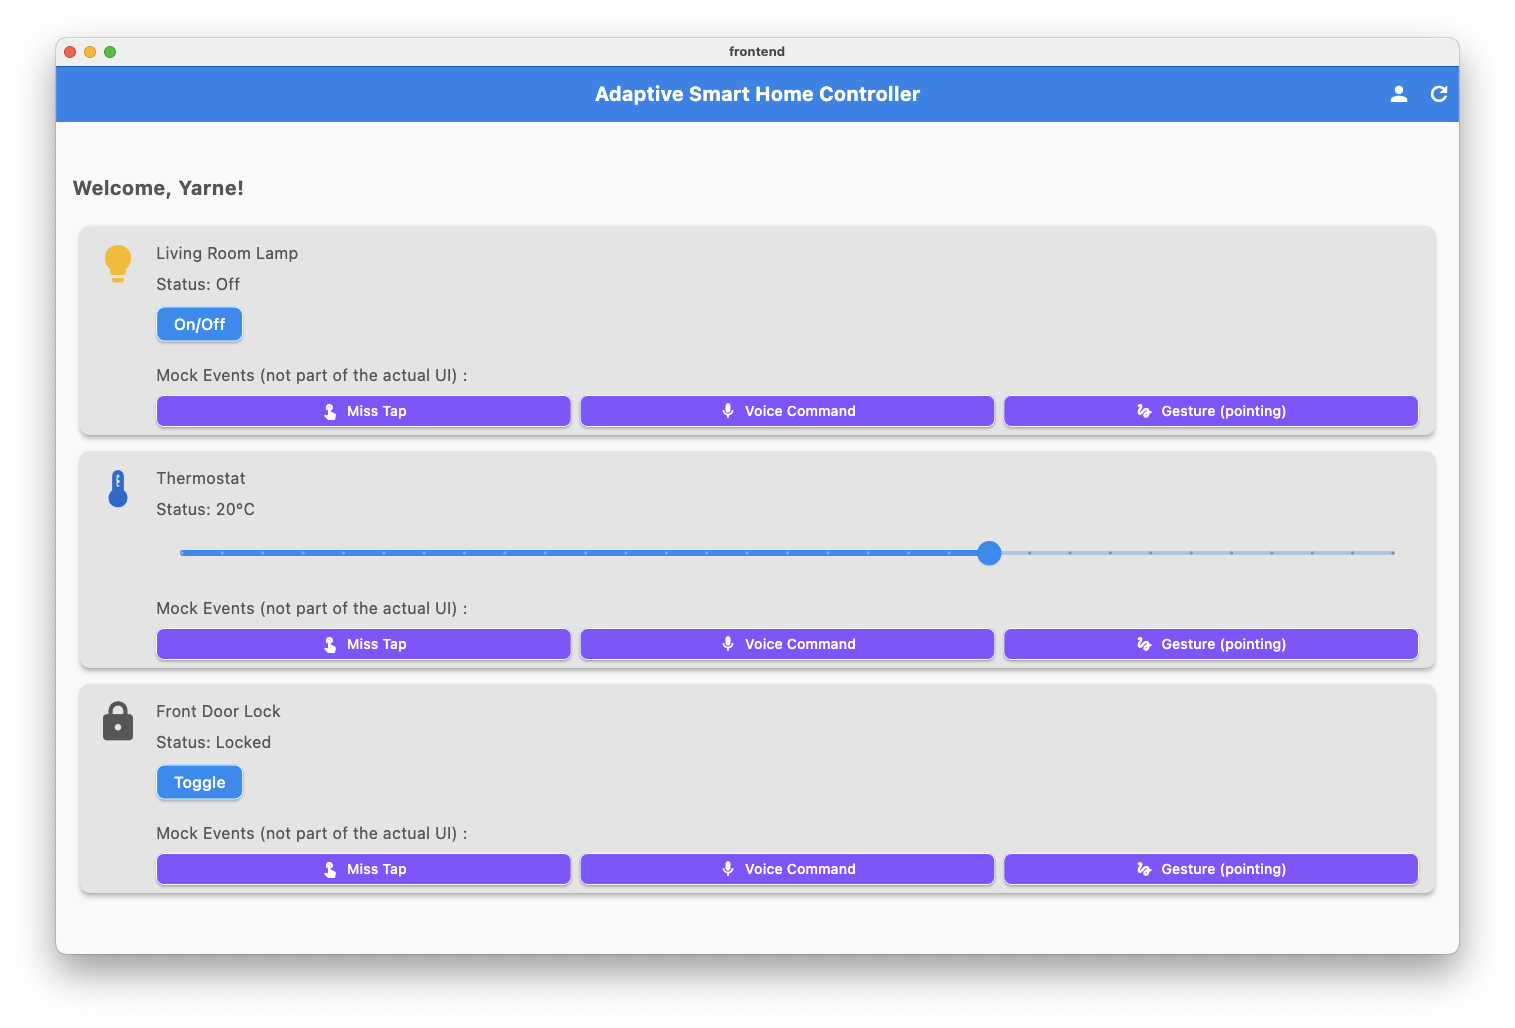
\includegraphics[width=\linewidth]{images/fig_ui_overview.png}
    \caption*{Before: standard interface with small targets}
\end{minipage}\hfill
\begin{minipage}{.5\linewidth}
    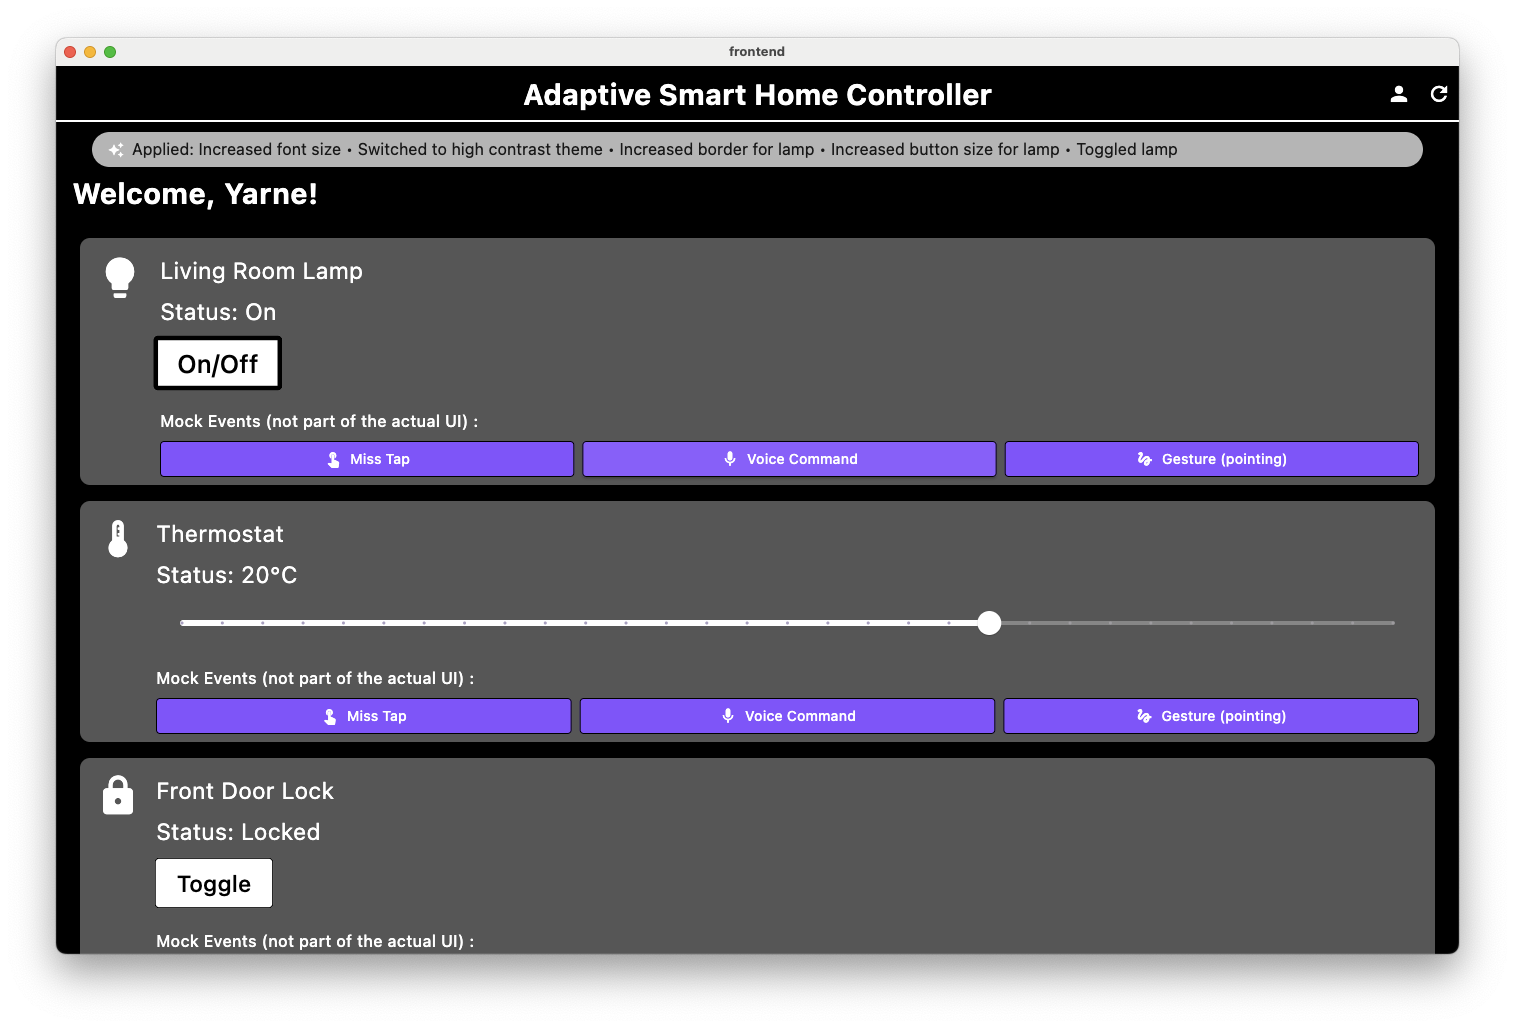
\includegraphics[width=\linewidth]{images/fig_adapt_after.png}
    \caption*{After: enlarged targets, enhanced contrast, stronger borders}
\end{minipage}
\caption{Real-time adaptation applied after miss-tap event for visually impaired user.}
\label{fig:before-after-adaptation}
\end{figure}

\section{Backend Injection Interface}

\subsection{Purpose and Scope}
This lightweight Flutter tool exposes a direct interface to the SIF backend for debugging and evaluation. It lets a researcher inject or edit \emph{profiles} and \emph{events}, send them to the backend over WebSocket/HTTP, and immediately inspect the returned \texttt{\{adaptations:[...]\}} along with the server-side interaction history per user. It is separate from the end-user UI and optimized for fast iteration. 

\subsection{Architecture and Data Flow}
On launch the app opens a WebSocket to \texttt{ws://localhost:8000/ws/adapt} and listens for JSON replies containing an \texttt{adaptations} array. Profile updates are sent via HTTP \texttt{POST /profile}, while the history panel pulls entries from \texttt{GET /full\_history}. Incoming WS frames are decoded and the \texttt{adaptations} list is rendered; after each reply the tool refreshes history via HTTP to keep the view in sync. 

\subsection{Controls: Profiles and Events}
The left column edits the \emph{profile} (free-form JSON or prefilled “Motor Impaired” / “Hands-Free”), visualizing key blocks like \texttt{accessibility\_needs} and \texttt{input\_preferences}. The right column edits the \emph{event} (free-form JSON or predefined “Miss-Tap on Play”, “Voice Play Command”, “Gesture Point”). Both editors pretty-print JSON and show an iconized summary (user, modality, target). This enables fast A/B of context vs. input without leaving the app (see figure \ref{fig:backend-inject-adapt-config} for an example).

\begin{figure}[h]
\centering
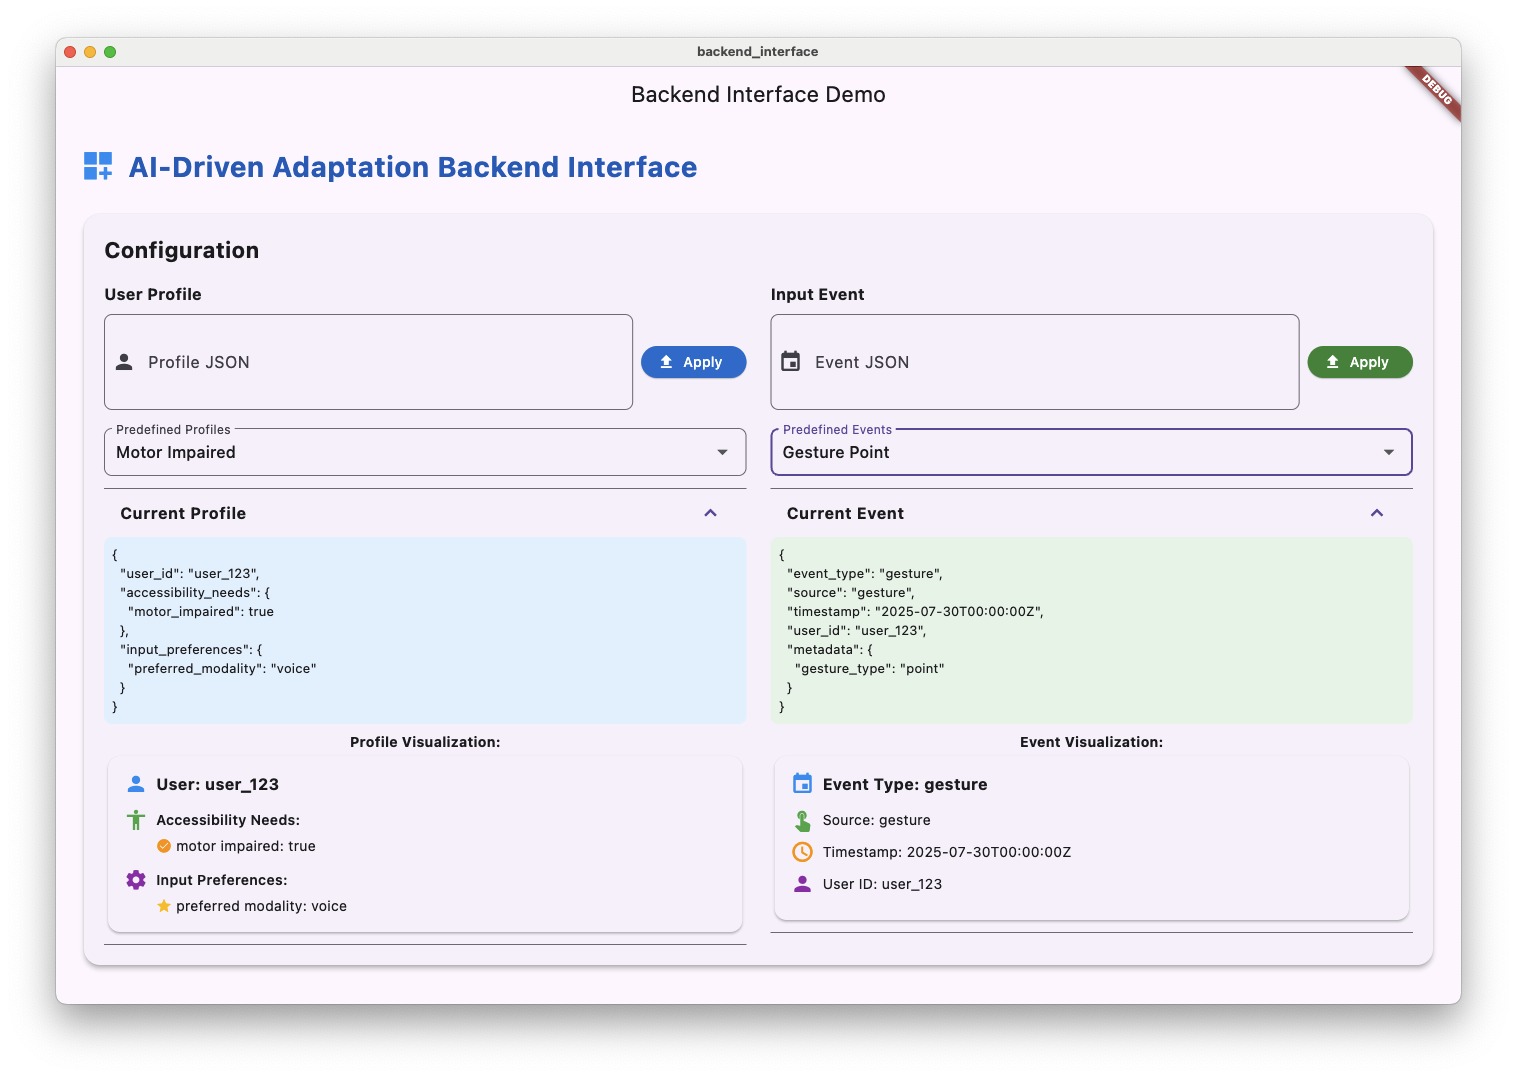
\includegraphics[width=.5\linewidth]{images/fig_backend_inject_config.png}\hfill
\caption{Backend Injection Interface: configuration and live JSON visualization.}
\label{fig:backend-inject-adapt-config}
\end{figure}

\subsection{Adaptation Response View}
Pressing \emph{Get Suggestions} sends the current event (after posting the profile), shows a spinner, then lists each adaptation with an action-specific icon and a compact, human-readable summary (e.g., “Switch to voice mode” or “Increase contrast”). The mapping covers common actions such as \texttt{switch\_mode}, \texttt{increase\_contrast}, \texttt{trigger\_button}, \texttt{simplify\_layout}, and geometry actions. Unknown actions fall back to a generic renderer, keeping the tool resilient to backend experiments (see figure \ref{fig:backend-inject-adapt} for an example). 

\begin{figure}[h]
\centering
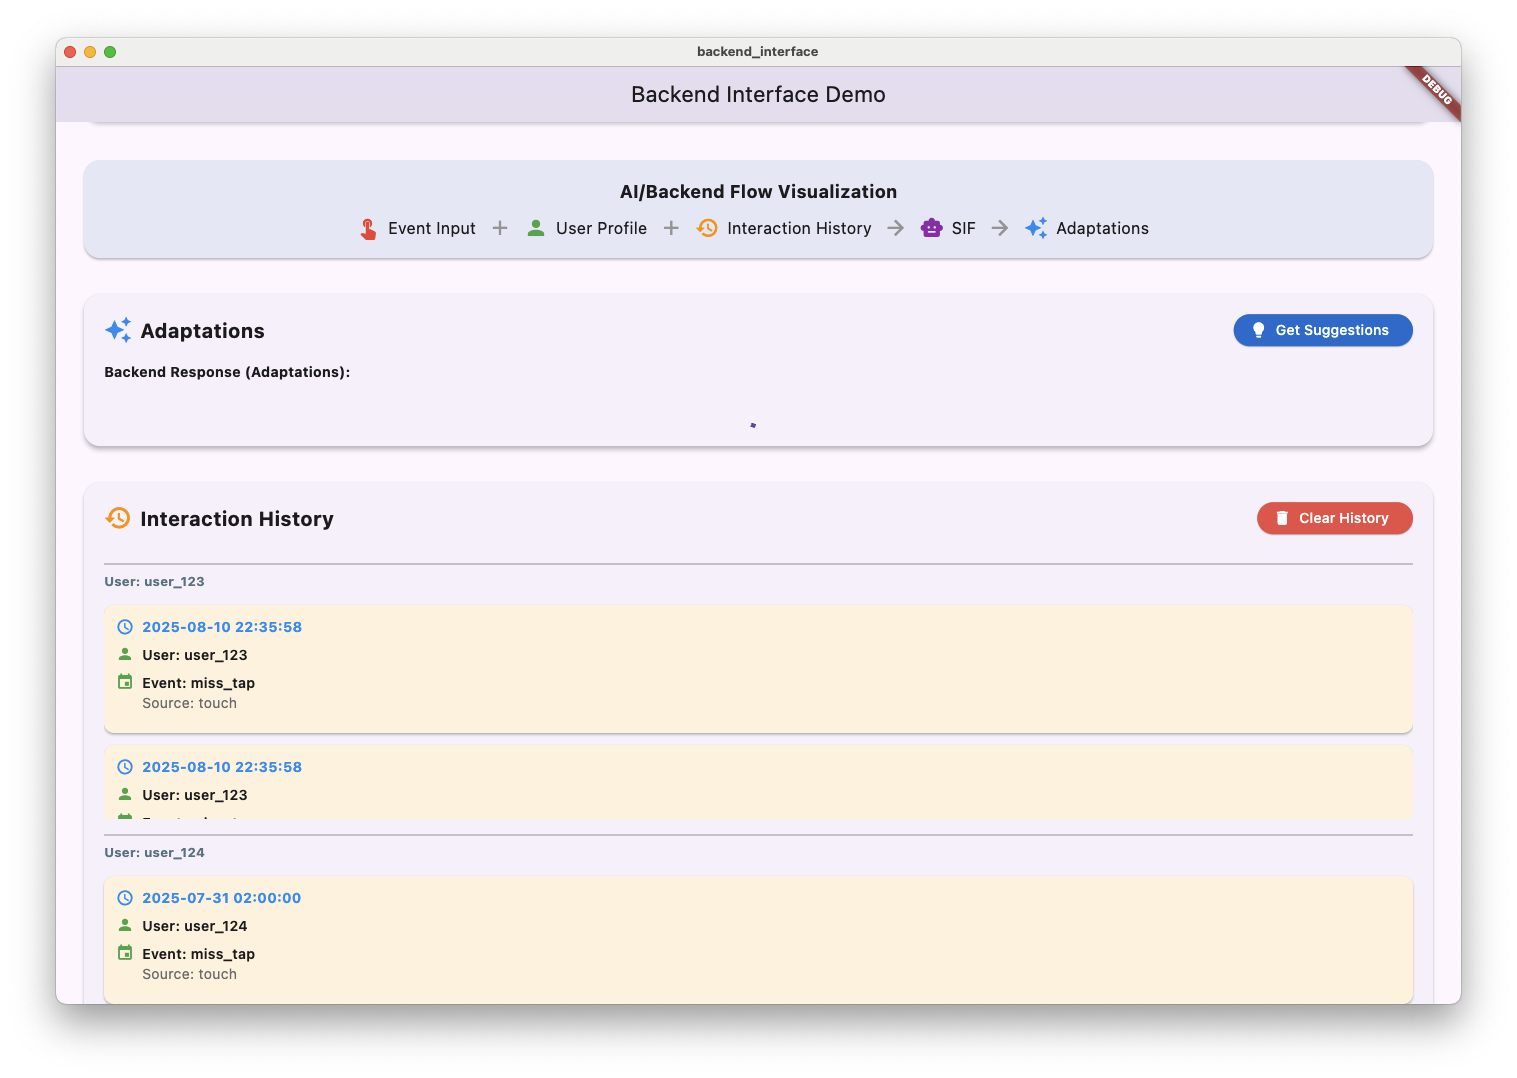
\includegraphics[width=.5\linewidth]{images/fig_backend_inject_adapt_before.png}\hfill
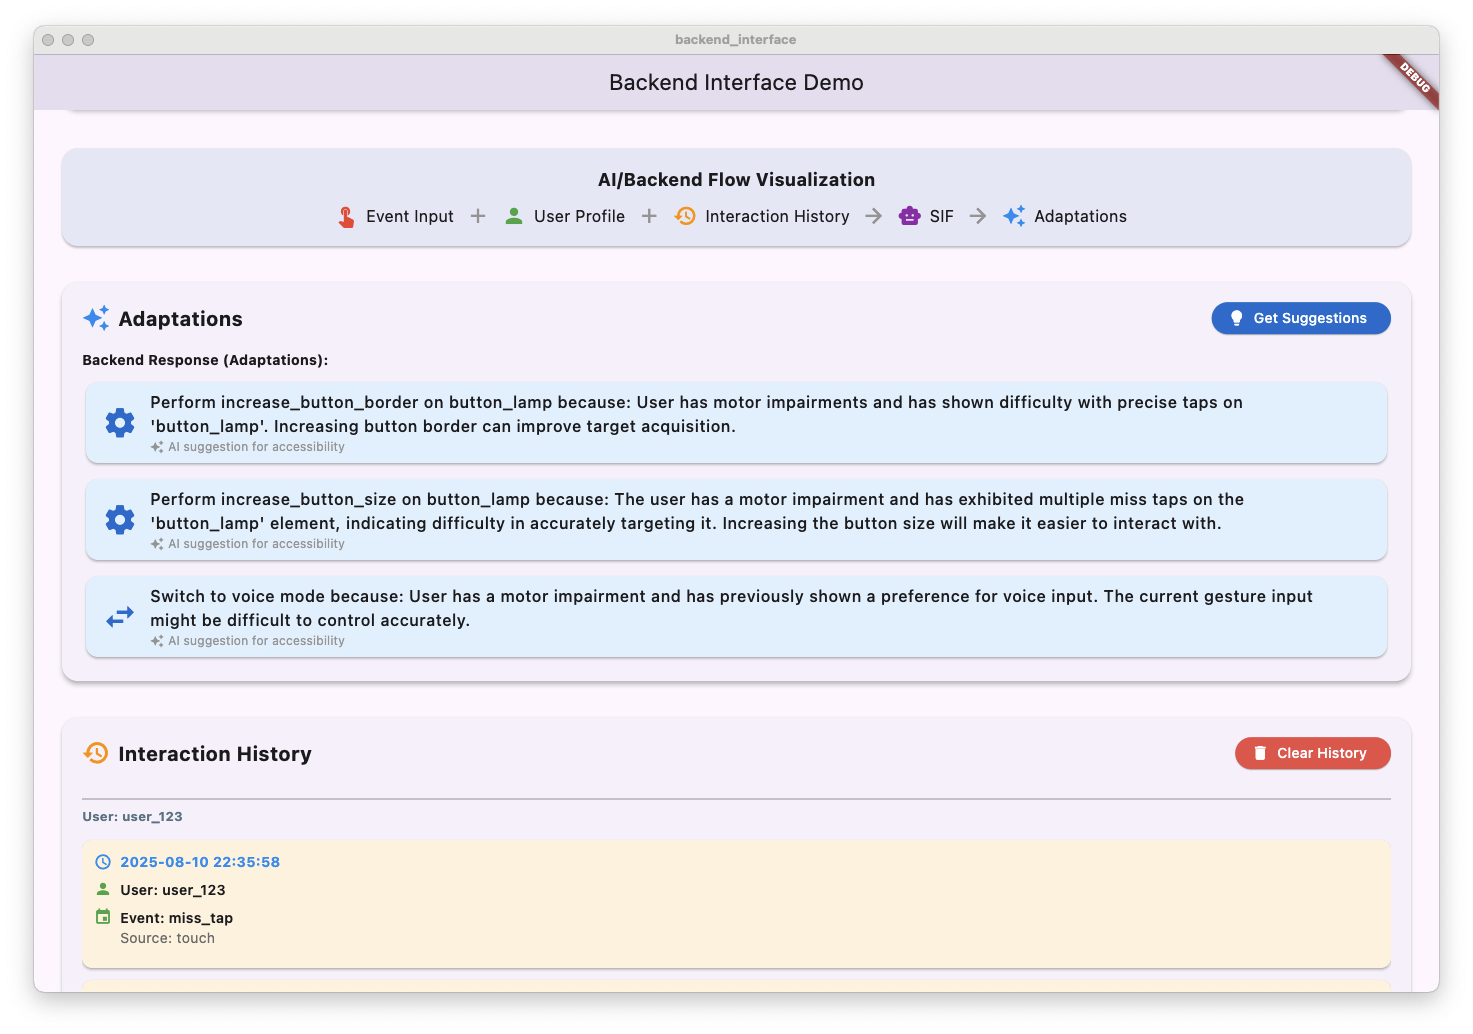
\includegraphics[width=.5\linewidth]{images/fig_backend_inject_adapt_after.png}
\caption{Example adaptation list before/after a pointing gesture event.}
\label{fig:backend-inject-adapt}
\end{figure}

\subsection{Interaction History Panel}
The bottom card fetches \texttt{history} from the backend and renders each entry (timestamp, user, event type/source) plus the associated adaptations. This provides a quick audit trail to verify that profile changes affect subsequent suggestions and to spot repeated error patterns (e.g., consecutive miss-taps). A “Clear History” button resets the local view; history retrieval is refreshed after each WS reply to keep causality visible.

\subsection{Operational Notes and Limitations}
The app assumes a running backend at \texttt{localhost:8000}. Profile JSON is posted verbatim; there is no schema validation beyond backend checks. The WS channel is established once on init; a commented reconnection helper is included for future hardening. Timeouts and transport errors are surfaced minimally to keep the UI uncluttered. This is created as a developer tool and is not intended for end-users.

\section{Cross-Platform SwiftUI Example}

\subsection{Purpose and Scope}
This minimal SwiftUI app demonstrates that a thin, platform-native adapter plus a small view layer are sufficient to integrate with the SIF backend. It mirrors the Flutter contract: create (or fetch) a user profile over HTTP, stream events over WebSocket, and apply the returned \texttt{\{adaptations:[...]\}} envelope to the UI state. The example targets iOS/macOS (Swift~5.7+, iOS~15+) and may require ATS exceptions for local HTTP/WS during development.

\subsection{Adapter and Transport}
The \texttt{AdaptiveUIAdapter} is an \texttt{ObservableObject} that (i) ensures the profile exists via \texttt{GET /profile/
\{user\_id\}} and \texttt{POST /profile}, (ii) opens a \texttt{URLSessionWebSocketTask} to \texttt{/ws/adapt}, and (iii) exposes \texttt{sendEvent(\,)} and an \texttt{onAdaptations} callback for the UI. Incoming frames are decoded from a wrapped
 \texttt{Envelope\{adaptations:[...]\}} into an array of \texttt{Adaptation}. On receive errors it reconnects after a short delay, keeping the session resilient for local testing and debugging. Events are encoded with \texttt{JSONEncoder.convertToSnakeCase}, matching the backend’s snake\_case contract.

\subsection{Minimal UI and State Mapping}
\texttt{AdaptiveUIApp} wires the adapter into the environment and renders a single \texttt{ContentView} that shows a lamp card, a few “send event” buttons, and a live list of the most recent adaptations (see figure \ref{fig:swift-adapt} for a before-after example). The view holds a small set of reactive states \texttt{buttonScale}, \texttt{borderWidth}, \texttt{highContrast}, \texttt{fontScale}, \texttt{spacing}, and \texttt{tooltip}, that the \texttt{apply(\,)} function updates based on \texttt{action}/\texttt{target}/\texttt{value}/\texttt{mode}. Concretely:  
\emph{increase\_button\_size} multiplies \texttt{buttonScale}, \emph{increase\_font\_size} scales text, \emph{increase\_contrast} toggles a high-contrast color scheme, \emph{increase\_button\_border} sets a visible outline, \emph{adjust\_spacing} scales inter-control spacing (clamped), \emph{show\_tooltip} surfaces the model’s reason string, and \emph{trigger\_button} toggles the lamp state. This mirrors the Flutter mapping but proves the contract is UI-framework agnostic. 

\subsection{Event Injection}
Three buttons generate representative events: a miss-tap (\texttt{event\_type="miss\_tap"} with coordinates), a simple voice command (\texttt{event\_type="voice"} with \texttt{metadata.command}), and a local tap. The miss-tap and voice paths serialize to JSON and are sent over WS; the tap path is stubbed to flip local state, emphasizing that production UIs would simply send the tap event the same way. 

\subsection{Usage and Limitations}
On launch, the adapter creates a minimal default profile when needed, connects WS, and begins listening. Pressing “Miss-tap” or “Voice” triggers a backend roundtrip; the adaptation list below the card updates immediately and \texttt{apply(\,)} mutates view state. The demo intentionally omits persistence and complex navigation; its goal is to show that the SIF contract (profile endpoints, WS envelope, action names) can be integrated cleanly into SwiftUI with \(\approx\)~a hundred lines of adapter+view code.

\begin{figure}[h]
\centering
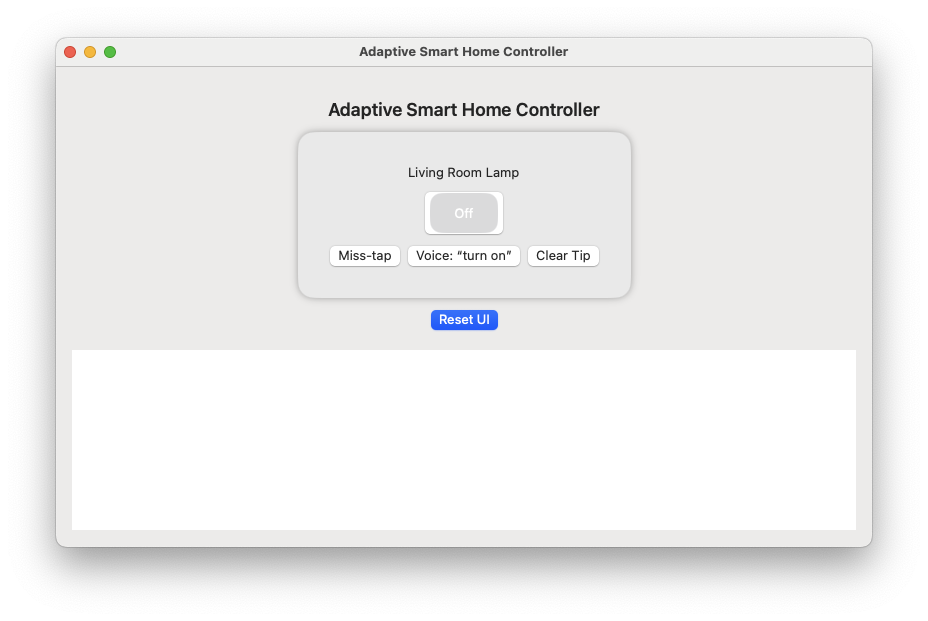
\includegraphics[width=.5\linewidth]{images/fig_swift_before.png}\hfill
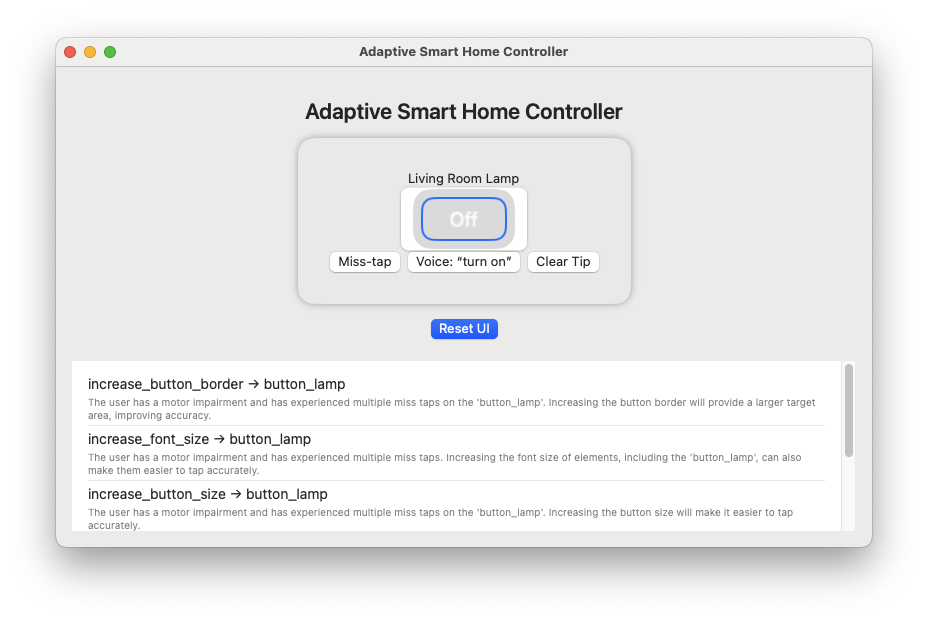
\includegraphics[width=.5\linewidth]{images/fig_swift_after.png}
\caption{Example SwiftUI app before/after a miss\_tap event.}
\label{fig:swift-adapt}
\end{figure}

\section{Design Decisions}
The design of the Adaptive Multimodal GUI Framework using LLMs reflects a series of deliberate choices aimed at balancing accessibility, performance, scalability, extensibility, and ease of integration. These decisions were made with the primary goal of delivering real-time, personalised adaptations for motor-impaired, visually impaired, and hands-free users, while ensuring that the framework remains modular and adaptable to future platforms and domains.

\subsection{Modularity Over Monolithic Design}
\textbf{Decision:} The framework adopts a modular three-layer architecture (Frontend, Input Adapter, SIF Backend) with clear separation of concerns, connected through a standardised JSON contract.

\textbf{Reasoning:}
\begin{itemize}
    \item \textbf{Flexibility:} Each layer can be updated or replaced independently, enabling deployment across different platforms such as Flutter, SwiftUI, or future platforms without reworking the entire system.
    \item \textbf{Extensibility:} The JSON contract in the Input Adapter Layer allows new modalities (e.g., eye tracking) to be integrated without modifying backend logic.
    \item \textbf{Developer accessibility:} Modularity simplifies integration, requiring minimal code for event handling and adaptation application.
\end{itemize}

\subsection{WebSocket for Real-Time vs. HTTP for Batch Processing}
\textbf{Decision:} The framework uses WebSocket (\texttt{/ws/adapt}) for real-time event processing and adaptation delivery, with HTTP (\texttt{/full\_history, /profile}) for debugging, developer tooling and profile management.

\textbf{Reasoning:}
\begin{itemize}
    \item \textbf{Low Latency:} WebSocket enables fast and bidirectional sending of data like adaptations (e.g., scaling a button after a miss-tap).
    \item \textbf{Reliability:} HTTP supports robust profile updates (\texttt{POST} \texttt{/profile}), ideal for non-real-time scenarios or debugging.
    \item \textbf{Accessibility:} Real-time feedback enhances usability for motor-impaired or hands-free users, where delays could disrupt interaction. 
\end{itemize}

\subsection{MongoDB for Persistent Storage}
\textbf{Decision:} MongoDB is used for storing user profiles, interaction history, and adaptation logs, with \texttt{user\_id} indexing and capped history arrays (10 events).

\textbf{Reasoning:}
\begin{itemize}
  \item \textbf{Scalability:} MongoDB’s NoSQL design and indexing ensure fast queries for large user bases, critical for real-world deployment.
  \item \textbf{Flexibility:} JSON-like documents align with the framework’s JSON contract, simplifying profile/history storage.
  \item \textbf{Continuous Learning:} Retaining a limited history supports adaptive behaviour, such as making permanent size adjustments after repeated miss-taps.
\end{itemize}

\subsection{Rule-Based Fallback with LLM Reasoning}
\textbf{Decision:} SIF combines rule-based logic (e.g., \texttt{if miss\_tap then increase\_size}) with LLM reasoning for creative adaptations, with rules as a fallback for LLM failures or time-outs, since LLM's can have high respond latencies.

\textbf{Reasoning:}
\begin{itemize}
  \item \textbf{Reliability:} Rules ensure deterministic adaptations (e.g., button enlargement for miss-taps) when LLM responses are unavailable or hallucinate.
  \item \textbf{Novelty:} LLM enables context-aware, proactive suggestions (e.g., \verb|switch_mode: voice| for hands-free users), advancing beyond static rules.
  \item \textbf{Accessibility:} Hybrid approach ensures consistent support for motor-impaired, visually impaired users (e.g., high-contrast text).
\end{itemize}

\subsection{Multi-agent LLM reasoning (MA-SIF) vs single-agent LLM reasoning (normal SIF)}
A key architectural decision in the framework is the adoption of multi-agent LLM reasoning (MA-SIF) over a single agent LLM approach (normal SIF). In the single agent SIF model, one LLM is responsible for interpreting all input events and generating adaptation actions. While this simplifies integration and reduces system complexity, it can limit the granularity and specialization of adaptation logic, especially as the diversity of user needs and input modalities grows.

MA-SIF, by contrast, distributes reasoning across multiple specialized LLM agents, each focused on a distinct domain such as UI adaptations, geometry/layout changes, input modality management, and validation. This separation of concerns enables each agent to leverage tailored prompts, domain-specific knowledge, and focused reasoning strategies, resulting in more nuanced and context-aware adaptation suggestions. The validator agent further ensures that outputs from other agents are coherent, non-conflicting, and accessibility-compliant.

The multi-agent approach offers several advantages: \begin{itemize} \item \textbf{Scalability:} New agents can be added to address emerging modalities or adaptation domains without disrupting existing logic. \item \textbf{Extensibility:} Prompts and allowed actions can be updated independently for each agent, supporting rapid iteration and domain-specific improvements. \item \textbf{Robustness:} Specialized agents reduce the risk of LLM hallucinations or conflicting adaptations, as validation is enforced before application. \item \textbf{Personalization:} Agents can incorporate user profiles and history more effectively, enabling targeted adaptations for motor-impaired, visually impaired, or hands-free users. \end{itemize}

\section{Implementation Challenges and Solutions}
Developing the Adaptive Smart Home Controller exposed several practical challenges, ranging from LLM-specific issues to general real-time system concerns. These were addressed through a mix of architectural decisions, fallback mechanisms, and compromises designed to keep the prototype functional and reliable under varying conditions.

\subsection{LLM reliability and output consistency}
One of the most persistent challenges was ensuring that the multi-agent LLM pipeline returned valid, schema-compliant output. Despite strict prompts and an explicit allowed-actions list, hallucinations still occurred, producing unsupported actions, targeting non-existent elements, or returning unreasonable values such as excessively large scaling factors. These errors risked breaking the layout or producing jarring visual changes. To mitigate this as described earlier, a validator agent was introduced to consolidate and correct suggestions before they reached the frontend. However, this validation step added extra latency and still could not guarantee complete protection against invalid values, making additional frontend-side checks a sensible next step for future versions.

\subsection{Performance under real-time constraints}
Adaptation latency was a critical factor for usability, particularly in accessibility scenarios where delayed feedback can reduce trust in the system. Smaller LLM models were assigned to the suggestion agents to keep their execution time within fractions of a second, while the validator, which required more context and reasoning, used a larger model with a higher timeout budget. Even so, occasional slowdowns occurred due to network latency or provider-side delays. The backend was therefore designed to apply partial results if all agents did not respond in time, ensuring that at least some adaptations reached the user quickly.

\subsection{Safeguards against malicious or replay attacks}
In its current form, the system does not include strong safeguards against replay attacks or intentionally crafted events designed to trigger disruptive adaptations. This is acceptable in a controlled research environment but would require strict validation and authentication for production deployment. Measures such as signing WebSocket messages, verifying sequence numbers, and rejecting stale or malformed events would be necessary to prevent exploitation as well as extra protections in the adapter or frontend. Furthermore is \texttt{user\_id} hijacking, where an attacker submits events under a different user’s profile possible, since no \texttt{user\_id} checks are done on returning adaptations. Future mitigations such as implementing \texttt{user\_id} verification and event signing will be necessary to address these vulnerabilities. This was intentional for the scope and development time constraints of this research.

\subsection{Testing with incomplete modalities}
Live gesture tracking and voice inputs were not integrated in this iteration, which meant that related adaptations had to be tested using simulated events. While this allowed the adaptation logic to be validated end-to-end, it did not account for the noise, recognition errors, or latency introduced by real input devices. Future work will need to focus on replacing these simulated events with actual input sources to fully evaluate performance in realistic conditions.

\subsection{Security and trust boundaries}
In its current implementation state, the backend accepts connections from any origin and does not require authentication for profile creation or event submission. Currently a pure localhost setup is implemented for the entire backend. This was a deliberate decision to speed up testing across platforms, but would need to be replaced with stricter CORS rules, token-based authentication, and access control in production. Without these measures, the system is vulnerable to unsolicited adaptation requests from external sources. Furthermore, some config files such as \texttt{sif\_config.json} do not have the necessary validation checks in the backend, while the validator agent is necessary, nothing stops it from being removed.

\section{Chapter Summary}
This chapter has detailed the implementation of the Adaptive Smart Home Controller as the primary proof-of-concept for the multimodal AI-driven GUI framework. The system was realised as a three-layer architecture, consisting of a Flutter-based frontend for rendering and applying adaptations, an Input Adapter Layer for standardising and transmitting events, and a FastAPI-based backend implementing multi-agent Smart Intent Fusion with MongoDB for persistent profile and history storage.

Key implementation aspects included the construction of a dynamic adaptation pipeline capable of applying size, contrast, modality, and content changes in real time, and the use of a strict JSON schema to maintain consistency between layers. While some modalities such as voice and gesture inputs were simulated for demonstration purposes, the system was designed so that integrating real devices will require minimal architectural changes.

The prototype also faced practical challenges, including LLM output validation, latency management, security considerations, and the absence of certain safeguards against malicious or replayed events. These were addressed through a combination of a validator agent, conservative rule-based fallbacks, partial-result handling, and a modular design that isolates critical components.

In its current state, the implementation demonstrates that the framework can deliver personalised, accessibility-focused adaptations in a responsive and modular manner, even under the constraints of a prototype environment. The next chapter evaluates this implementation through a feasibility study, assessing its responsiveness, adaptability, and practical potential in simulated real-world scenarios.
